\documentclass{article}

\usepackage[utf8]{vietnam}
\usepackage{graphicx}
\usepackage{setspace}
\usepackage{fancyhdr}

\counterwithin*{section}{part}

\usepackage[]{hyperref}
\usepackage{bookmark}
\hypersetup{
    colorlinks=true,
    linkcolor=black,
    filecolor=magenta,
    urlcolor=blue,
    pdftitle={Design Patterns - Final Exam Report},
    pdfpagemode=FullScreen,
}

\usepackage{tikz}
\usetikzlibrary{calc}

\usepackage[left=3.5cm,right=2cm,top=2cm,bottom=2cm]{geometry}

\usepackage{listings}
\usepackage{xcolor}

\definecolor{dkgreen}{rgb}{0,0.6,0}
\definecolor{gray}{rgb}{0.5,0.5,0.5}
\definecolor{mauve}{rgb}{0.58,0,0.82}

\lstset{frame=tb,
    language=Java,
    aboveskip=3mm,
    belowskip=3mm,
    showstringspaces=false,
    columns=flexible,
    numbers=left,
    numberstyle=\small\color{gray},
    keywordstyle=\color{blue},
    commentstyle=\color{dkgreen},
    stringstyle=\color{mauve},
    breaklines=true,
    breakatwhitespace=true,
    tabsize=3
}

\usepackage{titlesec}
\titlelabel{\thetitle.\quad}
\usepackage[dotinlabels]{titletoc}
\titlecontents{chapter}[1.5em]{\medskip\bfseries}%
{\contentslabel{1.7em}}
{}%numberless%
{\enspace\hfill\contentspage}[\smallskip]%

\dottedcontents{section}[2.5em]{\smallskip}{1.4em}{0.6pc}
\dottedcontents{subsection}[4.5em]{\smallskip}{2.3em}{0.6pc}

\usepackage[none]{hyphenat}
\tolerance=9999
\emergencystretch=10pt
\hyphenpenalty=10000
\exhyphenpenalty=100

%add some new paragraph command
\newcommand\para{\paragraph{} \hspace{0pt} \fontsize{13}{13}\selectfont \fontseries{b}\selectfont \indent}
\newcommand\subpara{\fontsize{13}{13}\selectfont \fontseries{b}\selectfont}
\newcommand\head{\fontsize{30}{20}\selectfont \fontseries{b}\selectfont}



\begin{document}
    \begin{tikzpicture}[overlay,remember picture]
        \draw [line width=2pt]
        ($ (current page.north west) + (3.0cm,-2.0cm) $)
        rectangle
        ($ (current page.south east) + (-2.0cm,2.5cm) $);
        \draw [line width=0.5pt]
        ($ (current page.north west) + (3.1cm,-2.1cm) $)
        rectangle
        ($ (current page.south east) + (-2.1cm,2.6cm) $);
    \end{tikzpicture}

    \begin{center}
        \pagenumbering{gobble}
        \fontsize{14}{20}\selectfont
        \textbf{ĐẠI HỌC QUỐC GIA HÀ NỘI\\
        \textbf{TRƯỜNG ĐẠI HỌC KHOA HỌC TỰ NHIÊN\\}
        \textbf{KHOA TOÁN - CƠ - TIN HỌC}}
        \vspace{0.8cm}
        \begin{figure}[htp]
            \begin{center}
                
\includegraphics[scale=0.5]{./image/logohus.png}
            \end{center}
        \end{figure}
        \fontsize{16}{20}\selectfont\textbf{BÁO CÁO CUỐI KỲ\\}
        \fontsize{20}{20}\selectfont\textbf{CÁC THÀNH PHẦN PHẦN MỀM\\}
        \vspace{1cm}
        \setstretch{1.5}
        \fontsize{18}{18}\selectfont\textbf{Tên Đề Tài: DESIGN PATTERNS}
        \textit{(nhóm 1)\\}
        \vspace{1cm}
    \end{center}

    \begin{flushleft}
        \fontsize{16}{20}\selectfont
        \textit{Sinh viên thực hiện:}\\
        \hspace{0.5cm}\textbf{Phạm Bá Thắng - 20001976}\\
        \hspace{0.5cm}\textbf{La Thị Anh Thư - 20001980}\\
    \end{flushleft}
    \vspace{3cm}
    \begin{center}
        \fontsize{14}{20}\selectfont
        \textbf{HÀ NỘI, 1/2022}
    \end{center}
    \pagebreak

    \pagestyle{fancy}
    \fancyhf{}
    \chead{\thepage}
    \renewcommand{\headrulewidth}{0pt}
    \begin{center}
        \head{LỜI CẢM ƠN}
        \hspace{15pt}
    \end{center}
    \para{Đầu tiên, chúng em xin gửi lời cảm ơn chân thành đến Trường Đại học Khoa học Tự nhiên đã đưa môn học Các thành phần phần mềm vào chương trình giảng dạy. Đặc biệt, chúng em xin gửi lời cảm ơn sâu sắc đến giảng viên bộ môn - Thầy Quản Thái Hà đã dạy dỗ, truyền đạt những kiến thức quý báu cho chúng em trong suốt thời gian học tập vừa qua. Trong thời gian tham gia lớp học Các thành phần phần mềm của thầy, chúng em đã có thêm cho mình nhiều kiến thức bổ ích, tinh thần học tập hiệu quả, nghiêm túc. Đây chắc chắn sẽ là hành trang để chúng em có thể vững bước sau này.}
    \para{Bộ môn Các thành phần phần mềm là môn học thú vị, vô cùng bổ ích và có tính thực tế cao. Đảm bảo cung cấp đủ kiến thức, gắn liền với nhu cầu phát triển của sinh viên. Tuy nhiên, khả năng tiếp nhận kiến thức của mỗi người luôn tồn tại những hạn chế nhất định. Do đó, bài báo cáo khó có thể tránh khỏi những thiếu sót. Kính mong thầy xem xét và góp ý để bài báo cáo của chúng em được hoàn thiện hơn.}
    \para{Kính chúc thầy sức khỏe, hạnh phúc, thành công trên con đường sự nghiệp giảng dạy. Những ngày cuối của năm cũ đang dần qua, chúng em chúc thầy năm mới vạn sự như ý, thêm một năm nữa đồng hành cùng các thế hệ sinh viên.}
    \pagebreak


    \begin{center}
        \head{Mục Lục}
    \end{center}
    \setstretch{1.5}
    \fontsize{13}{13}\selectfont
    \tableofcontents
    \pagebreak

    \pagenumbering{arabic}\setcounter{page}{1}\pagestyle{plain}

    \begin{center}
        \part{Tổng quát}
    \end{center}

    \section{Định nghĩa}
    \begin{itemize}
        \item[-]\subpara{Design pattern là một kỹ thuật lập trình quan trọng trong lập trình hướng đối tượng, cung cấp các khuôn mẫu thiết kế có thể dễ dàng áp dụng. Design pattern là các giải pháp tổng thể đã được tối ưu hóa, được tái sử dụng cho các vấn đề phổ biến trong thiết kế phần mềm mà chúng ta thường gặp phải hàng ngày. Đây là tập các giải pháp đã được suy nghĩ, đã giải quyết trong tình huống cụ thể và có thể dùng để giải quyết các vấn đề tương tự.}
    \end{itemize}

    \section{Đặc điểm}
    \begin{itemize}
        \item[-]\subpara{Design pattern có thể thực hiện được ở bất cứ ngôn ngữ lập trình nào sử dụng OOP. Nó giúp bạn giải quyết vấn đề một cách tối ưu nhất, cung cấp cho bạn các giải pháp trong lập trình hướng đối tượng (OOP).}
        \item[-]\subpara{Việc có khuôn mẫu sẵn nên tốc độ lập trình tăng, chỉ cần hiểu và áp dụng, không cần nghiên cứu mới; những người cùng team lập trình cũng dễ đọc dễ hiểu hơn, giảm bớt rủi ro do chưa được tối ưu hay có lỗi do nghiên cứu chưa hoàn thiện nên bớt tốn kém thời gian.}
        \item[-]\subpara{Tái sử dụng tối đa các mã nguồn, dễ dàng trong việc nâng cấp bảo trì để đáp ứng nhu cầu dự án.}
    \end{itemize}

    \section{Phân loại}
    \begin{itemize}
        \item[-]\subpara{Design pattern gồm 23 loại được chia thành 3 nhóm:}
        \begin{itemize}
            \item[+]\subpara{Creational Pattern (nhóm khởi tạo) gồm: Factory Method, Abstract Factory, Builder, Prototype, Singleton. Những Design pattern loại này cung cấp một giải pháp để tạo ra các object và che giấu được logic của việc tạo ra nó, thay vì tạo ra object một cách trực tiếp bằng cách sử dụng method new. Điều này giúp cho chương trình trở nên mềm dẻo hơn trong việc quyết định object nào cần được tạo ra trong những tình huống được đưa ra.}
            \item[+]\subpara{Structural Pattern (nhóm cấu trúc) gồm: Adapter, Bridge, Composite, Decorator, Facade, Flyweight và Proxy. Những Design pattern loại này liên quan tới class và các thành phần của object. Nó dùng để thiết lập, định nghĩa quan hệ giữa các đối tượng.}
            \item[+]\subpara{Behavioral Pattern (nhóm hành vi) gồm: Interpreter, Template Method, Chain of Responsibility, Command, Iterator, Mediator, Memento, Observer, State, Strategy và Visitor. Nhóm này dùng trong thực hiện các hành vi của đối tượng, sự giao tiếp giữa các object với nhau.}
        \end{itemize}
        \item[-]\subpara{Mối quan hệ giữa các design pattern:}
        \begin{figure}[htp]
            \begin{center}
                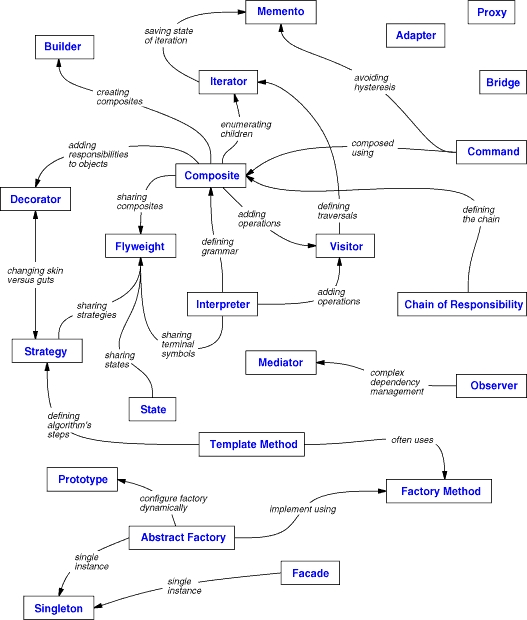
\includegraphics[scale=0.65]{./image/design-patterns-relationship.jpg}
            \end{center}
        \end{figure}
    \end{itemize}
    \pagebreak
    \begin{center}
        \hspace{0pt}
        \vfill
        \part{Nhóm Khởi tạo - Creational Pattern}
        \begin{figure}[htp]
            \begin{center}
                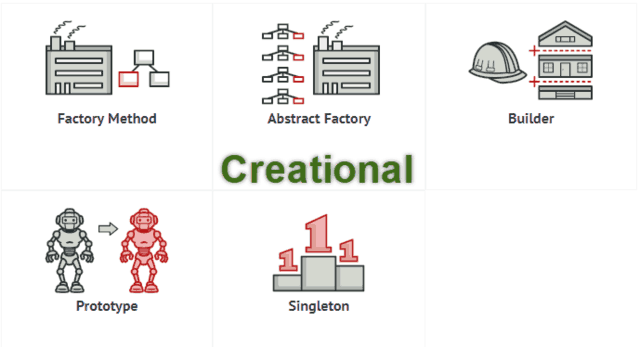
\includegraphics[scale=0.65]{./image/creational-pattern.png}
            \end{center}
        \end{figure}
        \vfill
        \hspace{0pt}
    \end{center}

    \pagebreak

    \section{Singleton}
    \subsection{Định Nghĩa Và Mô Hình Cấu Trúc}
    \begin{itemize}
        \item[-]\subpara{Singleton được thiết kế để đảm bảo chỉ duy nhất một instance được tạo ra và cung cấp một method để có thể truy xuất được instance đó mọi lúc mọi nơi trong chương trình.}
        \item[-]\subpara{Singleton ẩn đi hàm dựng của class và sử dụng các hàm có sẵn bên trong để tạo đối tượng.}
    \end{itemize}
    \begin{figure}[htp]
        \begin{center}
            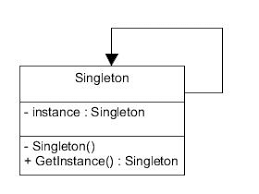
\includegraphics[scale=1]{./image/singleton-pattern.png}
        \end{center}
    \end{figure}

    \subsection{Đặc điểm}
    \begin{itemize}
        \item[-]\subpara{Đảm bảo rằng một lớp chỉ có một instance}
        \item[-]\subpara{Dễ dàng truy cập vào instance này}
        \item[-]\subpara{Kiểm soát việc khởi tạo nó}
        \item[-]\subpara{Giới hạn số lượng instance}
        \item[-]\subpara{Có thể truy cập như một biến toàn cục}
    \end{itemize}
    \subsection{Mục Đích Sử Dụng}
    \begin{itemize}
        \item[-]\subpara{Là dạng class nên có thể sử dụng với nhiều design pattern khác nhau}
        \item[-]\subpara{Sử dụng làm biến toàn cục với các ưu điểm như:}
        \begin{itemize}
            \item[+]\subpara{Không làm rối loạn danh sách các biến toàn cục vì không tạo ra các biến không cần thiết}
            \item[+]\subpara{Chúng cho phép phân bổ và khởi tạo khi cần (call-by-need), trong khi tạo nhiều các biến toàn cục ngay từ đầu sẽ luôn tiêu tốn tài nguyên}
        \end{itemize}
        \item[-]\subpara{Ví dụ như dùng để ghi log rất thích hợp vì chúng ta chỉ cần một bản ghi log duy nhất cho mỗi phiên, đồng thời điều này lại cần ở tất cả các bộ phận của chương trình}
    \end{itemize}

    \subsection{Code khuôn mẫu}
    \begin{lstlisting}
    public class Singleton {
        private static final Singleton INSTANCE = new Singleton();
        private Singleton() {}
        public static Singleton getInstance(){
            if(INSTANCE == null){
                INSTANCE = new Singleton();
            }
            return INSTANCE;
        }
    }
    \end{lstlisting}

    \subsection{Giải thích Design Pattern}
    \begin{itemize}
        \item[-]\subpara{Theo mô hình}
        \begin{itemize}
            \item[+]\subpara{Private constructor để hạn chế truy cập từ class bên ngoài.}
            \item[+]\subpara{Đặt private static final variable đảm bảo biến chỉ được khởi tạo trong class và duy nhất một lần.}
        \end{itemize}
        \item[-]\subpara{Theo code khuôn mẫu}
        \begin{itemize}
            \item[+]\subpara{Có một method public static để return instance được khởi tạo ở trên và một đoạn if để kiểm tra xem instance tồn tại chưa, nếu chưa sẽ gọi hàm khởi tạo. Hàm này được gọi là accessor.}
            \item[+]\subpara{Sau đó là các hàm để sử dụng.}
        \end{itemize}
    \end{itemize}

    \subsection{Ví Dụ Sử Dụng Trong Thực Tế}
    \begin{itemize}
        \item[-]\subpara{Ví dụ sử dụng Singleton pattern Simple Logger
        \\\href{https://github.com/blaplafla13th/design-patterns/tree/main/src/singleton}{https://github.com/blaplafla13th/design-patterns/tree/main/src/singleton}}
        \begin{figure}[htp]
            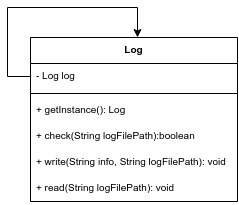
\includegraphics[scale=1]{./image/singleton-example.png}
        \end{figure}
        \item[-]\subpara{Tạo một logger theo Singleton pattern, sau đó chúng ta thêm các hàm kiểm tra file (check), hàm ghi file (write) và hàm đọc file (read). Khi runtime, các Exception được ghi lại và chuyển sang String rồi ghi ra file, sau đó file được đọc. Khi dùng trong package, người dùng có thể gọi các  hàm read, write và chỉ cần gọi đối tượng mà không cần khởi tạo lại đối tượng Log.}
        \item[-]\subpara{Đầu tiên tạo một biến thành viên hằng private là 1 instance Log mới và hàm dựng private của Log để giới hạn được số lượng đối tượng được tạo chỉ có duy nhất một đối tượng.}
        \item[-]\subpara{Tạo accessor getInstance với if để kiểm tra xem đối tượng Log có null không, nếu null thì tạo lại, sau đó trả về đối tượng Log được khai báo ở trên. Ta thêm các biến thành viên phục vụ cho việc ghi file như File, ghi ngày như SimpleDateFormat.}
        \item[-]\subpara{Hàm check sẽ kiểm tra xem file được truyền vào qua tham số có tồn tại không, không tồn tại thì sẽ tạo file mới, hai hàm read và write sẽ đọc và ghi file theo đường dẫn nhập từ tham số.}
        \item[-]\subpara{Sang bên test, chúng ta gọi đối tượng Log bằng cách sử dụng getInstance. Khai báo hằng LOG\_PATH để ghi đường dẫn của file log. Tạo thử 1 lỗi, sau đó ghi lỗi này ra log bằng lệnh write rồi đọc lại bằng lệnh read.}
    \end{itemize}
    \pagebreak

    \section{Builder}
    \subsection{Định Nghĩa Và Mô Hình Cấu Trúc}
    \begin{itemize}
        \item[-]\subpara{Builder là mẫu thiết kế được tạo ra để chia việc khởi tạo một đối tượng phức tạp thành từng phần riêng rẽ, từ đó có thể tiến hành khởi tạo đối tượng phức tạp này từ các đối tượng đơn giản hơn.}
        \item[-]\subpara{Mô hình:}
    \end{itemize}
    \begin{figure}[htp]
        \begin{center}
            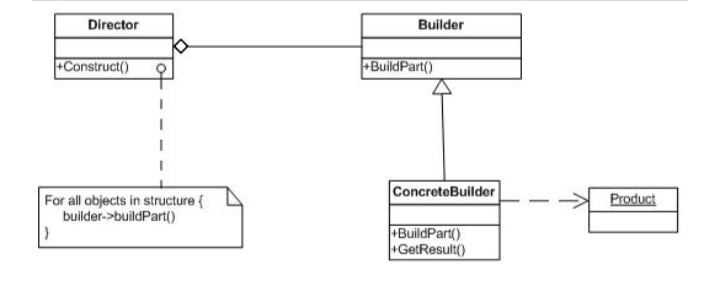
\includegraphics[scale=0.65]{./image/builder-pattern.jpg}
        \end{center}
    \end{figure}

    \subsection{Đặc điểm}
    \begin{itemize}
        \item[-]\subpara{Không cần truyền giá trị null cho các tham số không sử dụng}
        \item[-]\subpara{Kiểm soát tốt hơn quá trình khởi tạo đối tượng}
        \item[-]\subpara{Có thể tạo đối tượng immutable}
    \end{itemize}

    \subsection{Mục Đích Sử Dụng}
    \begin{itemize}
        \item[-]\subpara{Tạo một đối tượng phức tạp: có nhiều thuộc tính (nhiều hơn 4) và một số bắt buộc, một số không bắt buộc}
        \item[-]\subpara{Tách rời quá trình khởi tạo một đối tượng phức tạp từ các phần tạo nên đối tượng đó}
        \item[-]\subpara{Khi người dùng (client) mong đợi nhiều cách khác nhau cho đối tượng được khởi tạo}
        \item[-]\subpara{Giảm bớt số lượng hàm constructor}
    \end{itemize}


    \subsection{Code khuôn mẫu}
    \begin{lstlisting}
//Builder.java
public interface Builder {
    public void buildPartOne();
    public void buildPartTwo();
    public Product getProduct();
}

//Client.java
public class Client {
    public static void main(String[] args) {
        Director director = new Director(new ConcreteBuilder());
        director.makeProduct();

        Product product = director.getProduct();

        System.out.println("Product part: " + product.getPartOne());
        System.out.println("Product part: " + product.getPartTwo());
    }
}

//ConcreteBuilder.java
public class ConcreteBuilder implements Builder{
    private Product product;

    public ConcreteBuilder() {
        this.product = new Product();
    }

    @Override
    public void buildPartOne() {
        product.setPartOne("Part One");
    }

    @Override
    public void buildPartTwo() {
        product.setPartTwo("Part Two");
    }

    @Override
    public Product getProduct() {
        return product;
    }
}

//Director.java
public class Director {
    private Builder builder;

    public Director(Builder builder){
        this.builder = builder;
    }

    public void makeProduct(){
        builder.buildPartOne();
        builder.buildPartTwo();
    }

    public Product getProduct(){
        return builder.getProduct();
    }
}

//Product.java
public class Product {
    private String partOne;
    private String partTwo;

    public String getPartOne() {
        return partOne;
    }

    public void setPartOne(String partOne) {
        this.partOne = partOne;
    }

    public String getPartTwo() {
        return partTwo;
    }

    public void setPartTwo(String partTwo) {
        this.partTwo = partTwo;
    }
}
    \end{lstlisting}

    \subsection{Giải thích Design Pattern}
    \begin{itemize}
        \item[-]\subpara{Theo mô hình}
        \begin{itemize}
            \item[+]\subpara{Product: đại diện cho đối tượng cần tạo, đối tượng này phức tạp, có nhiều thuộc tính.}
            \item[+]\subpara{Builder: là abstract class hoặc interface khai báo phương thức khởi tạo đối tượng.}
            \item[+]\subpara{ConcreteBuilder: kế thừa Builder và cài đặt chi tiết cách tạo ra đối tượng. Nó sẽ xác định và nắm giữ các instance mà nó tạo ra, đồng thời nó cũng cung cấp phương thức để trả về các  mà nó đã tạo ra trước đó. Hay nói cách khác là bản thiết kế từng bước của đối tượng Product}
            \item[+]\subpara{Director/Client: là nơi sẽ gọi tới Builder để tạo ra đối tượng.}
        \end{itemize}
        \item[-]\subpara{Theo code khuôn mẫu}
        \begin{itemize}
            \item[+]\subpara{Khi chạy main của Client, đối tượng Director được khởi tạo, với đối đầu vào là một instance ConcreteBuilder được kế thừa từ Builder chứa thông tin từng bước.}
            \item[+]\subpara{Tiếp theo Client sẽ gọi hàm thực thi trong Director là hàm makeProduct chứa các bước trong interface builder rồi từ đó gọi các hàm override bởi các hàm trong Builder ConcreteBuilder để thực hiện các bước khởi tạo đối tượng.}
            \item[+]\subpara{Sau khi Director dựng xong đối tượng, Client lấy đối tượng Product về từ Director, từ đó có thể sử dụng Product như bình thường.}
        \end{itemize}
    \end{itemize}

    \subsection{Ví Dụ Sử Dụng Trong Thực Tế}
    \begin{itemize}
        \item[-]\subpara{Hệ thống quản lý tài khoản sử dụng builder pattern\\ \href{https://github.com/blaplafla13th/design-patterns/tree/main/src/builder}{https://github.com/blaplafla13th/design-patterns/tree/main/src/builder}}
        \begin{figure}[htp]
            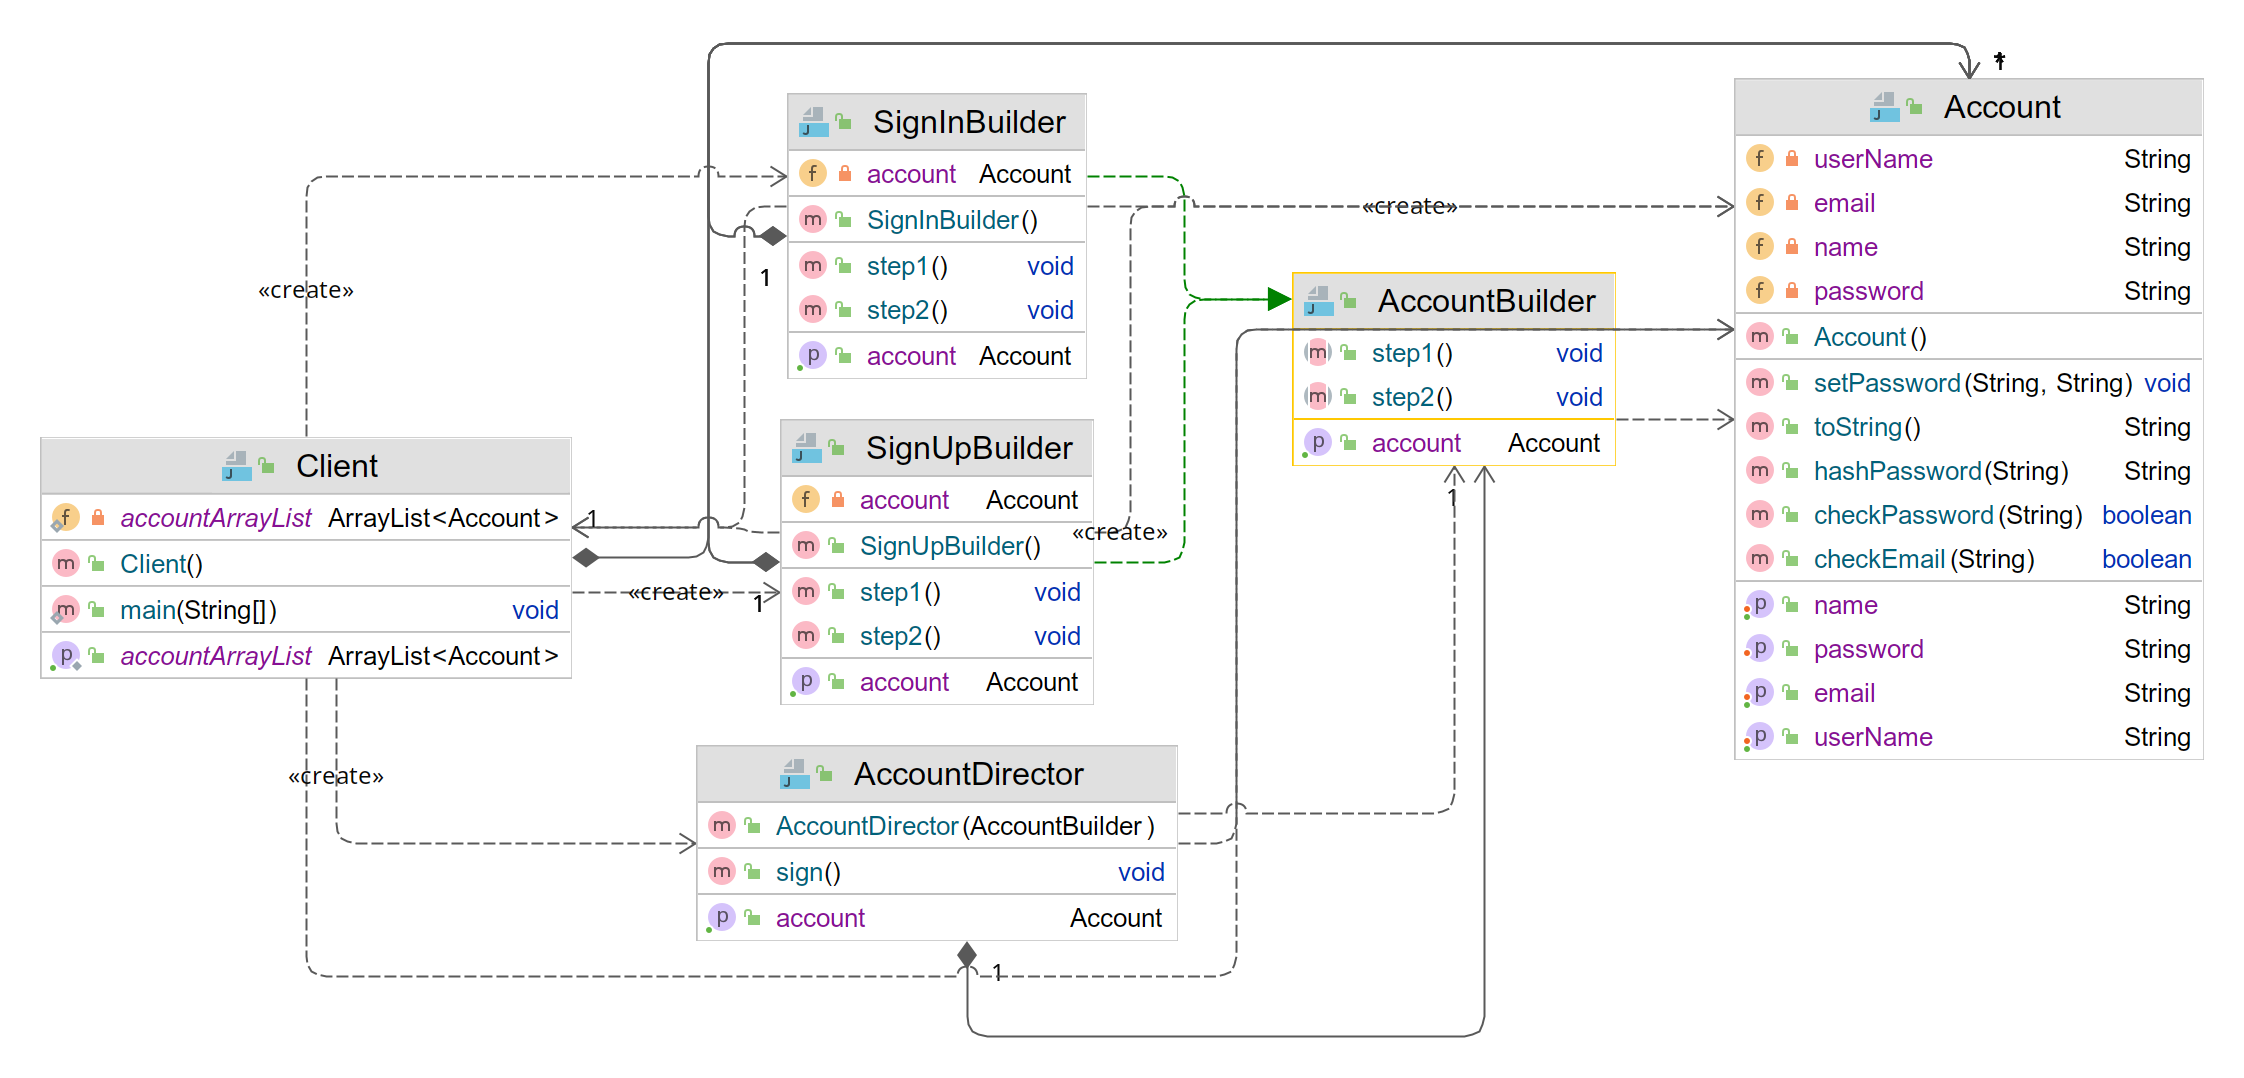
\includegraphics[scale=0.21]{./image/builder-example.png}
        \end{figure}
        \item[-]\subpara{Tài khoản (Account) gồm các thuộc tính cơ bản như userName, password, email name. Trong class account có getter và setter cho 4 thuộc tính trên, ngoài ra còn có những hàm phụ.}
        \item[-]\subpara{Khi tạo tài khoản hay đăng nhập, chúng ta có hai bước là ghi nhận thông tin và xử lý thông tin. Như vậy chúng ta cần tạo một interface AccountBuilder đóng vai trò builder với 2 step để xử lý, trong đó step 1 có vai trò điền thông tin, step 2 sẽ xử lý dữ liệu và đọc ghi vào mảng cụ thể là accountArrayList ở Client.java. Tiếp theo tạo class kế thừa AccountBuilder của signIn và signUp đóng vai trò ConcreteBuilder để tạo form điền ở step1 và xử lý form ở step2.}
        \item[-]\subpara{Chúng ta tạo một AccountDirector đóng vai trò Director tạo đối tượng builder để chạy hai builder vừa tạo. Hàm dựng sẽ nhận bản thiết kế của class builder và thực hiện các bước. Sau đó là hàm để return đối tượng.}
        \item[-]\subpara{Về phía Client, ta cần tạo 1 arraylist để lưu tài khoản và hàm để gọi arraylist này đặt tên là accountArrayList và thêm một hàm getter cho nó. Trong thực tế sẽ được lưu trong cơ sở dữ liệu, ở đây để đơn giản, dùng arraylist. Trong main ta tạo biến current để lưu tài khoản hiện tại đóng vai trò quản lý phiên. Tạo một vòng lặp để lựa chọn đăng kí hoặc đăng nhập và 2 director tương ứng với 2 lựa chọn này. Tiếp theo chúng ta sẽ chạy hàm sign của Director để Director chạy các bước như thiết kế.}
        \item[-]\subpara{Như vậy ta hoàn toàn có thể đọc sửa thông tin của account như ví dụ ở Client và khi lưu chúng ta set current vào index thay thế cho account hiện đăng nhập. Khi log out chúng ta đặt current = null để thoát phiên.}
    \end{itemize}
    \pagebreak

    \section{Factory}
    \subsection{Định Nghĩa Và Mô Hình Cấu Trúc}
    \begin{itemize}
        \item[-]\subpara{Factory Pattern hay Factory Method sử dụng một interface hay một abstract class mà tất cả các lớp chúng ta cần khởi tạo đối tượng sẽ kế thừa. Factory sẽ khởi tạo và trả về các đối tượng theo yêu cầu, giúp cho việc khởi tạo đối tượng một cách linh hoạt hơn. Nôm na Factory như phân xưởng sản xuất một sản phẩm.}
        \item[-]\subpara{Abstract Factory là bản mở rộng của Factory khi object chúng ta khởi tạo bao gồm nhiều object khác liên quan. Trong Abstract Factory pattern, một interface có nhiệm vụ tạo ra các Factory của các object có liên quan tới nhau mà không cần phải chỉ ra trực tiếp các class của object. Nôm na Abstract Factory như một nhà máy với nhiều phân xưởng là các Factory Method.}
        \item[-]\subpara{Mô hình cho Factory:}
        \begin{figure}[htp]
            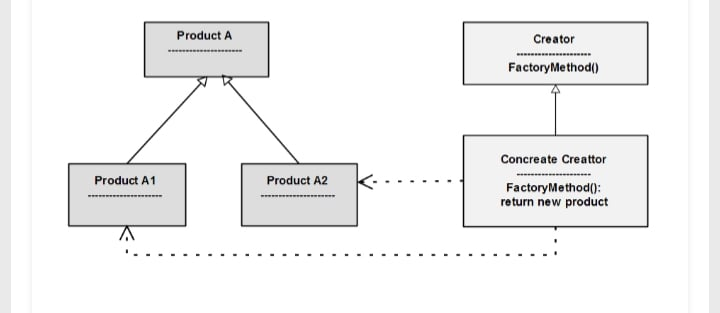
\includegraphics[scale=0.7]{./image/factory-pattern.jpg}
        \end{figure}
    \end{itemize}
    \subsection{Đặc điểm}
    \begin{itemize}
        \item[-]\subpara{Người dùng không biết logic thực sự được khởi tạo bên dưới phương thức factory như thế nào}
        \item[-]\subpara{Cho phép các lớp con chọn kiểu đối tượng cần tạo}
        \item[-]\subpara{Code chỉ tương tác với interface hoặc lớp abstract}
        \item[-]\subpara{Dễ dàng quản lý file cycle của các đối tượng được tạo}
        \item[-]\subpara{Thống nhất về mặt naming convention}
    \end{itemize}

    \subsection{Mục Đích Sử Dụng}
    \begin{itemize}
        \item[-]\subpara{Tạo ra cách mới trong việc khởi tạo đối tượng thông qua một interface chung}
        \item[-]\subpara{Che giấu đi xử lý logic của việc khởi tạo đối tượng}
        \item[-]\subpara{Giảm sự phụ thuộc giữa các module và tăng tính mở rộng code}
        \item[-]\subpara{Khi Factory có quá nhiều trường hợp, sử dụng Abstract Factory giúp phân tách điều kiện đơn giản hóa logic. Theo như mô hình ở dưới, AbtractFactory sẽ lựa chọn ConcreteFactory kế thừa từ mình để tạo ra Product}
        \item[-]\subpara{Mô hình cho Abstract Factory:}
        \begin{figure}[htp]
            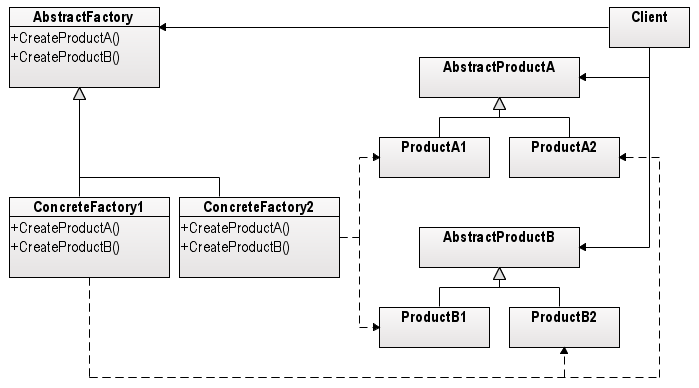
\includegraphics[scale=0.7]{./image/abstract-factory-pattern.png}
        \end{figure}
    \end{itemize}


    \subsection{Code khuôn mẫu}
    \begin{lstlisting}
//Factory.java
public class Factory {
    public Product createProduct(String productType){
        switch (productType){
            case "a": return new ProductA();
            case "b": return new ProductB();
            ...
            default: return null;
        }
    };
}

//Product.java
public abstract class Product {
    ...
}

//ProductA.java
public class ProductA extends Product{
    public ProductA(){
        ...
    }
    ...
}

//ProductB, ... similar as class ProductA

//Client.java
public class Client{
    public static void main(String[] args){
        Factory factory = new Factory();
        Product product = factory.createProduct("a");
    }
}
    \end{lstlisting}

    \subsection{Giải thích Design Pattern}
    \begin{itemize}
        \item[-]\subpara{Theo mô hình}
        \begin{itemize}
            \item[+]\subpara{Super Class: môt super class (class A trong mô hình) trong Factory Pattern có thể là một interface, abstract class hay một class thông thường. các Sub Class (A1, A2,...) là các class kế thừa từ class A theo nhiệm vụ của nó.}
            \item[+]\subpara{Class ConcreteCreator hay Factory sẽ chịu tránh nhiệm khởi tạo các đối tượng sub class dựa theo tham số đầu vào và trả về cho Client. Thường thì class này là 1 Singleton.}
            \item[+]\subpara{Sau đó class Client hay Creator sẽ gọi đến Concrete Creator để lấy đối tượng mà chúng ta cần.}
            \item[+]\subpara{Đối với Abstract Factory, sẽ có nhiều Factory ConcreteCreator hay hơn kế thừa từ AbstractFactory. Client sẽ yêu cầu AbstractFactory và AbstractFactory sẽ gọi đến Factory tương ứng để thực hiện các hàm dựng các đối tượng theo chỉ định.}
        \end{itemize}
        \item[-]\subpara{Theo code khuôn mẫu}
        \begin{itemize}
            \item[+]\subpara{Chúng ta có 1 superclass Product và các class con kế thừa class Product như ProductA, ProductB,...}
            \item[+]\subpara{Class Factory có nhiệm vụ tạo đối tượng với 1 hàm createProduct trong đó tham số là loại product. Trong hàm là 1 switch case để khi nhập 1 giá trị, hàm sẽ trả về 1 đối tượng mới tương ứng của Product.}
            \item[+]\subpara{Về phía Client, chúng ta tạo một instance của Factory rồi dùng hàm createProduct từ đối tượng factory để tạo ra đối tượng mình mong muốn.}
        \end{itemize}
    \end{itemize}

    \subsection{Ví Dụ Sử Dụng Trong Thực Tế}
    \begin{itemize}
        \item[-]\subpara{Hệ thống thanh toán đơn giản sử dụng factory pattern \\ \href{https://github.com/blaplafla13th/design-patterns/tree/main/src/factory}{https://github.com/blaplafla13th/design-patterns/tree/main/src/factory}}
        \item[-]\subpara{Chúng ta tạo 1 package paymentmethod để chứa interface PaymentMethod và các class implements từ PaymentMethod. Mỗi class đều chứa tên phương thức, số tài khoản, tên người dùng và đoạn code ẩn để thanh toán.}
        \item[-]\subpara{Tiếp theo tạo 1 class FactoryPaymentMethod chứa 1 hàm trả về đối tượng PaymentMethod với đối đầu vào là tên phương thức thanh toán và bên trong chứa 1 switch case các phương thức thanh toán. Mỗi lựa chọn của switch case trả về 1 instance PaymentMethod tương ứng.}
        \item[-]\subpara{Đối với Client ta dùng hàm listFile để gọi ra các phương thức thanh toán khả dụng trong package paymentmethod. Khi người dùng nhập phương thức thanh toán, đối tượng factoryPaymentMethod được khởi tạo, chạy hàm getPaymentMethod để trả về phương thức thanh toán như yêu cầu. Từ đó người dùng có thể sử dụng các hàm trong phương thức thanh toán mà không biết nó được khởi tạo như thế nào bên dưới phương thức factory.}
        \item[-]\subpara{Khi cần thêm phương thức thanh toán, lập trình viên chỉ cần tạo 1 class mới trong package paymentmethod và thêm vào switch case của FactoryPaymentMethod.}
        \begin{figure}[htp]
            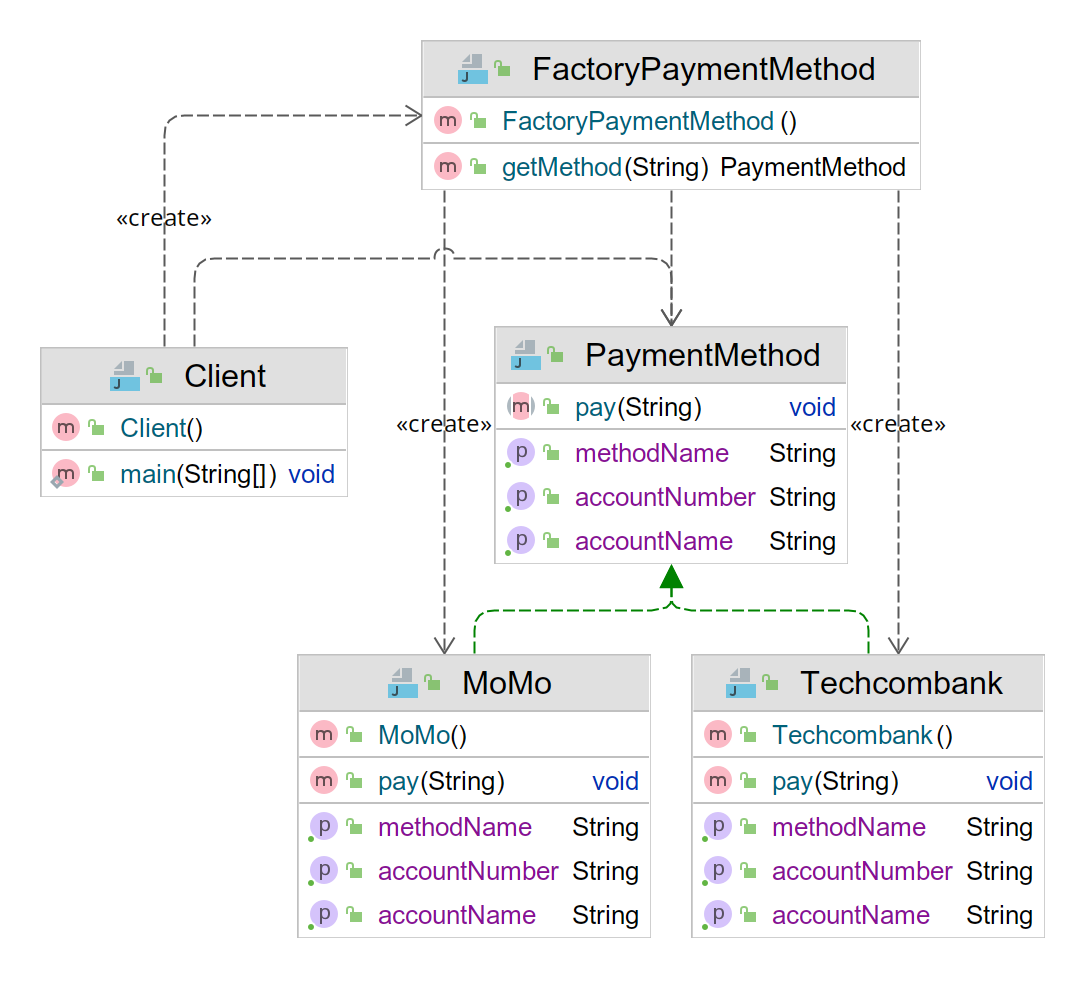
\includegraphics[scale=0.4]{./image/factory-example.png}
        \end{figure}
    \end{itemize}
    \pagebreak

    \begin{center}
        \hspace{0pt}
        \vfill
        \part{Nhóm Cấu trúc - Structural Pattern}
        \begin{figure}[htp]
            \begin{center}
                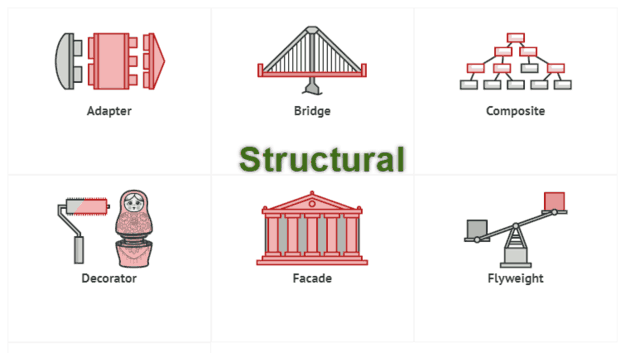
\includegraphics[scale=0.65]{./image/structural-pattern.png}
            \end{center}
        \end{figure}
        \vfill
        \hspace{0pt}
    \end{center}
    \pagebreak

    \section{Adapter}
    \subsection{Định Nghĩa Và Mô Hình Cấu Trúc}
    \begin{itemize}
        \item[-]\subpara{Adapter Pattern cho phép các interface không liên quan tới nhau có thể làm việc cùng nhau. Đối tượng giúp kết nối các interface gọi là Adapter.}
        \item[-]\subpara{Adapter Pattern giữ vai trò trung gian giữa hai lớp, chuyển đổi interface của một hay nhiều lớp đã có sẵn thành một interface khác, thích hợp cho lớp đang viết.}
        \item[-]\subpara{Mô hình:}
    \end{itemize}
    \begin{figure}[htp]
        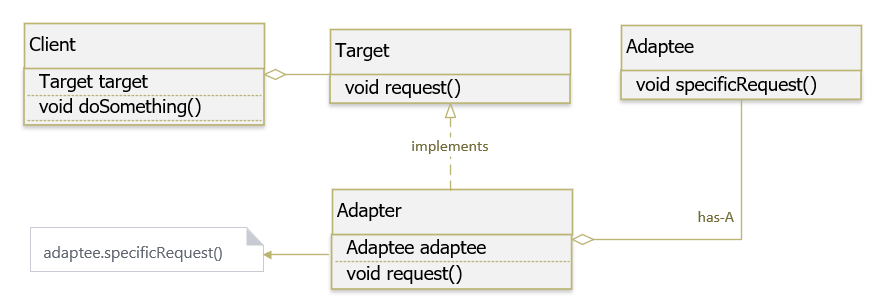
\includegraphics[scale=0.5]{./image/adapter-pattern.png}
    \end{figure}

    \subsection{Đặc điểm}
    \begin{itemize}
        \item[-]\subpara{Phân tách việc chuyển đổi interface với business logic chính của chương trình}
        \item[-]\subpara{Có thể sử dụng adapter với các class con của adaptee}
        \item[-]\subpara{Làm việc với adapter class thay vì sửa đổi bên trong adaptee class đã có sẵn}
        \item[-]\subpara{Client tiếp cận thông qua interface thay vì implementation}
        \item[-]\subpara{Tăng chi phí và độ phức tạp của code}
    \end{itemize}

    \subsection{Mục Đích Sử Dụng}
    \begin{itemize}
        \item[-]\subpara{Chuyển đổi interface của một class thành interface mà client yêu cầu}
        \item[-]\subpara{Tạo ra những lớp có khả năng sử dụng lại, chúng phối hợp với các lớp không liên quan hay những lớp không thể đoán trước được và những lớp này không có interface tương thích}
        \item[-]\subpara{Khi muốn đảm bảo nguyên tắc Open/Close trong một ứng dụng}
    \end{itemize}


    \subsection{Code khuôn mẫu}
    \begin{lstlisting}
//Adaptee.java
public class Adaptee {
    ...
    public void specificRequest() {
        ...
    }
}

//Adapter.java
public class Adapter implements Target {
    private Adaptee adaptee;

    public Adapter(Adaptee adaptee){
        this.adaptee = adaptee;
    }

    @Override
    public void request() {
        adaptee.specificRequest();
    }
}

//Client.java
public class Client {
    public static void main(String[] args) {
        Target target = new Adapter(new Adaptee());
        target.request();
    }
}

//Target.java
public interface Target {
    public void request();
}
    \end{lstlisting}

    \subsection{Giải thích Design Pattern}
    \begin{itemize}
        \item[-]\subpara{Theo Mô hình}
        \begin{itemize}
            \item[+]\subpara{Adaptee: là một class hoặc interface không tương thích, cần được tích hợp vào trong client.}
            \item[+]\subpara{Adapter: lớp tích hợp, giúp class không tương thích tích hợp được với interface đang làm việc. Thực hiện việc chuyển đổi interface cho Adaptee và kết nối Adaptee với Client. Adapter thường chứa adaptee hoặc kế thừa từ adaptee. Các phương thức không cần thiết sẽ bị interface ẩn đi. Nếu adaptee là 1 object chứa bên trong adapter, adapter có thể làm được nhiều việc với nhiều adaptee hơn thay vì chỉ một adapter với 1 adaptee.}
            \item[+]\subpara{Target: một interface chứa các chức năng được sử dụng bởi Client.}
            \item[+]\subpara{Client: lớp sử dụng các đối tượng có interface Target.}
        \end{itemize}
        \item[-]\subpara{Theo code khuôn mẫu}
        \begin{itemize}
            \item[+]\subpara{Class Adaptee có 1 phương thức cần.}
            \item[+]\subpara{Một interface Target sẽ chứa hàm request với mục đích để gọi hàm trong Adaptee.}
            \item[+]\subpara{Adapter sẽ implements interface Target, có một hàm dựng với tham số là instance của Adaptee. Hàm request của Adapter sẽ gọi đến hàm cần yêu cầu của Adaptee.}
            \item[+]\subpara{Client: sẽ tạo instance của Adapter với đối số là một đối tượng adaptee mới. Như vậy ta có thể gọi hàm cần yêu cầu qua phương thức request trên target.}
        \end{itemize}
    \end{itemize}

    \subsection{Ví Dụ Sử Dụng Trong Thực Tế}
    \begin{itemize}
        \item[-]\subpara{Dịch một chương trình đơn giản bằng adapter pattern\\
        \href{https://github.com/blaplafla13th/design-patterns/tree/main/src/adapter}{https://github.com/blaplafla13th/design-patterns/tree/main/src/adapter}}
        \begin{figure}[htp]
            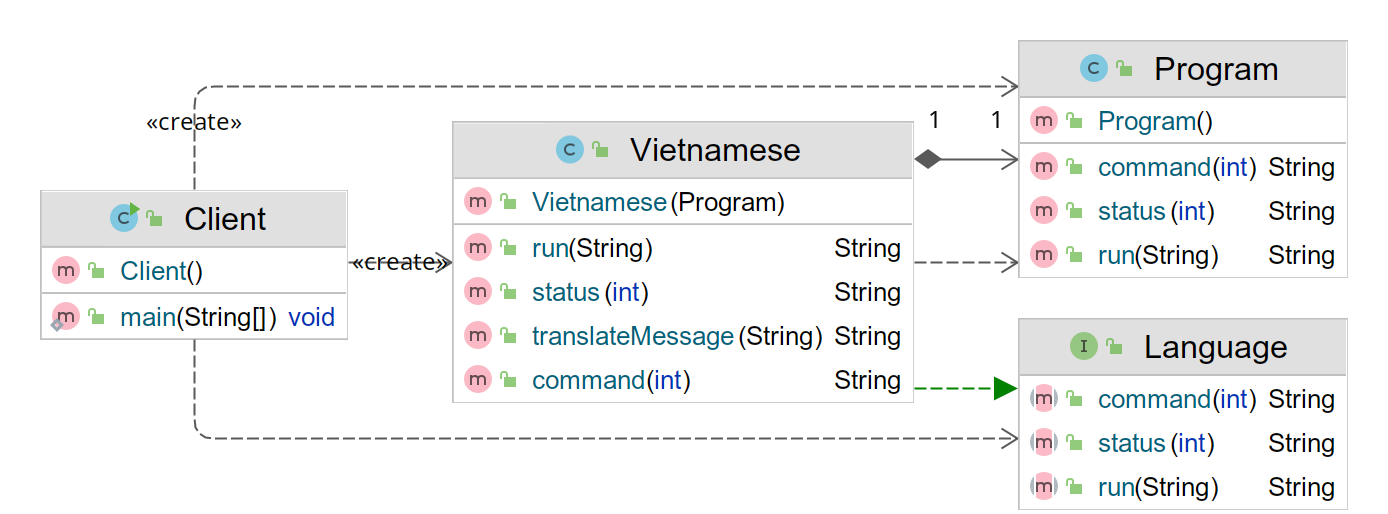
\includegraphics[scale=0.37]{./image/adapter-example.png}
        \end{figure}
        \item[-]\subpara{Ban đầu chúng ta có 2 file Program.java và Client.java. Program.java sử dụng hàm command và status để trả về các giá trị String rồi mới in chứ không in trực tiếp String bằng System.out.println. Class Program ở đây đóng vai trò của adaptee, giờ chúng ta sẽ viết 1 adapter Language và target Vietnamese.}
        \item[-]\subpara{Ta tạo một interface Language chứa các hàm sẽ gọi của Program trong main làm target.}
        \item[-]\subpara{Tạo một class implememt interface Language ở đây là class Vietnamese. Trong class ta sẽ dùng mảng String 2 chiều để lưu cặp giá trị String gồm từ chương trình trả về và từ chúng ta muốn dịch sang (mảng languagePack). Viết hàm translateMessage với tham số kiểu String để nhận giá trị chương trình trả về. Tạo 1 vòng for để tìm giá trị đó trong languagePack và trả về giá trị tương ứng của cặp.}
        \item[-]\subpara{Trong các hàm implement từ Language chúng ta sẽ trả về giá trị mà translateMessage trả về từ tham số tương ứng với đối số truyền vào là kết quả của hàm tương ứng bên file Program.java\\ Ví dụ như hàm run trong Vietnamese sẽ lấy tham số truyền vào giống hàm run ở Program trả về là translateMessage với đối số truyền vào là kết quả trả về của hàm run bên Program.}
        \item[-]\subpara{Đối với Client.java, chúng ta tạo một instance kiểu Language của class Vietnamese với đối số truyền vào là Program và thay vì gọi đến hàm trong instance Program thì chúng ta gọi đến instance của Language. Hay đơn giản hơn thay vì chúng ta sửa dòng tạo đối tượng Program thành tạo đối tượng kiểu  Language của class Vietnamese, đối số là đối tượng Program mới, giữ nguyên tên biến là ta đã dịch thành công chương trình.}
        \item[-]\subpara{Trong thực tế cách này được dùng kết hợp với factory pattern để dịch các chương trình sử dụng bộ các keyword:value để in thông tin, keyword:value thường được lưu ra file riêng, sẽ có hàm đọc file này để ghi vào mảng languagePack ở trên, cách này không dịch được các thông tin cứng được in trực tiếp mà không có trong bộ keyword:value.}
    \end{itemize}
    \pagebreak

    \section{Bridge}
    \subsection{Định Nghĩa Và Mô Hình Cấu Trúc}
    \begin{itemize}
        \item[-]\subpara{Bridge Pattern tách tính trừu tượng (abstraction) ra khỏi tính hiện thực (implementation) của nó. Từ đó, có thể dễ dàng chỉnh sửa hoặc thay thế mà không làm ảnh hưởng đến những nơi có sử dụng lớp ban đầu.}
        \item[-]\subpara{Mô hình:}
    \end{itemize}
    \begin{figure}[htp]
        \begin{center}
            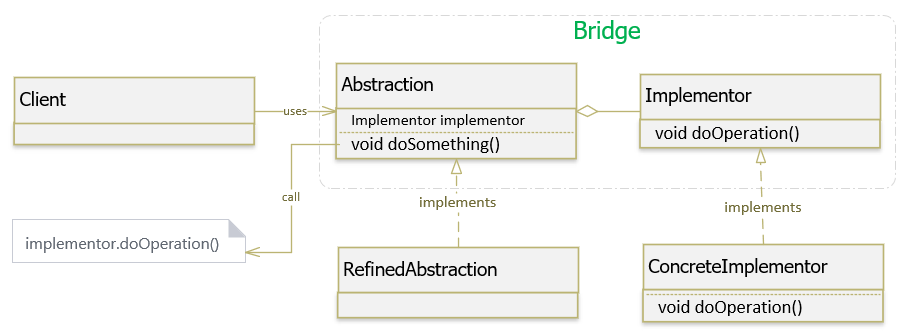
\includegraphics[scale=0.5]{./image/bridge-pattern.png}
        \end{center}
    \end{figure}

    \subsection{Đặc điểm}
    \begin{itemize}
        \item[-]\subpara{Giảm sự phụ thuộc giữa abstraction và implementation}
        \item[-]\subpara{Abstraction và implementation thay vì liên hệ bằng quan hệ kế thừa thì sẽ liên hệ với nhau thông qua object composition}
        \item[-]\subpara{Cho phép ẩn các chi tiết implement từ client}
        \item[-]\subpara{Dễ bảo trì và mở rộng về sau}
    \end{itemize}

    \subsection{Mục Đích Sử Dụng}
    \begin{itemize}
        \item[-]\subpara{Tách ràng buộc giữa abstraction và implementation để có thể dễ dàng mở rộng độc lập nhau}
        \item[-]\subpara{Thay đổi được thực thi trong implement mà không ảnh hưởng đến phía client}
    \end{itemize}

    \subsection{Code khuôn mẫu}
    \begin{lstlisting}
//Abstraction.java
public interface Abstraction {
	void operation();
}

//Client.java
public class Client {
	public static void main(String[] args) {
        Abstraction[] abstractions = new Abstraction[2];
        abstractions[0] = new RefinedAbstraction(new ImplementorA());
        abstractions[1] = new RefinedAbstraction(new ImplementorB());

        for(Abstraction abstraction:abstractions) {
            abstraction.operation();
        }
    }
}

//ImplementorA.java
public class ImplementorA implements Implementor{
	public void operation() {
        System.out.println("This is implementation");
    }
}

//ImplementorB, ... similar as class ImplementorA

//Implementor.java
public interface Implementor {
	void operation();
}

//RefinedAbstraction.java
public class RefinedAbstraction implements Abstraction{
    private Implementor implementator;

    public RefinedAbstraction(Implementor implementator){
        this.implementator = implementator;
    }

    public void operation(){
        implementator.operation();
    }
}
    \end{lstlisting}

    \subsection{Giải thích Design Pattern}
    \begin{itemize}
        \item[-]\subpara{Theo Mô hình }
        \begin{itemize}
            \item[+]\subpara{Client: đại diện cho khách hàng sử dụng các chức năng thông qua Abstracion.}
            \item[+]\subpara{Abstraction : định ra một abstract interface quản lý việc tham chiếu đến đối tượng hiện thực cụ thể (Implementor).}
            \item[+]\subpara{RefinedAbstraction (AbstractionImpl) : hiện thực (implement) các phương thức đã được định ra trong Abstraction bằng cách sử dụng một tham chiếu đến một đối tượng của Implementor.}
            \item[+]\subpara{Implementor : định ra các interface cho các lớp hiện thực. Thông thường nó là interface định ra các tác vụ nào đó của Abstraction.}
            \item[+]\subpara{ConcreteImplementor : hiện thực Implementor interface.}
        \end{itemize}
        \item[-]\subpara{Theo code khuôn mẫu}
        \begin{itemize}
            \item[+]\subpara{Client tạo 1 mảng Abstraction, mỗi phần tử của Abstraction tạo một instance của RefinedAbstraction sau đó gọi operation từ từng phần tử.}
            \item[+]\subpara{Interface Abstraction chứa hàm operation để sử dụng ở Client. RefinedAbstraction implements từ Abstraction. Trong RefinedAbstraction có 1 object thành viên là Implementor. Hàm operation kế thừa từ Implementor sẽ chạy hàm operation của Implementor.}
            \item[+]\subpara{Interface Implementor chứa khuôn mẫu hàm chạy của các Implementor. Các ImplementorA, B... implement từ Implemention.}
            \item[+]\subpara{Khi Client chạy, mảng Abstraction được khởi tạo, tạo mới Implementor làm đối của hàm dựng RefinedAbstraction. Khi Client gọi operation của Abstraction, RefinedAbstraction sẽ gọi đến operation của Implementor.}
        \end{itemize}
    \end{itemize}

    \subsection{Ví Dụ Sử Dụng Trong Thực Tế}
    \begin{itemize}
        \item[-]\subpara{Sử dụng bridge pattern để tạo chương trình hoạt động trên đa nền tảng\\
        \href{https://github.com/blaplafla13th/design-patterns/tree/main/src/brigde}{https://github.com/blaplafla13th/design-patterns/tree/main/src/brigde}}
        \begin{figure}[htp]
            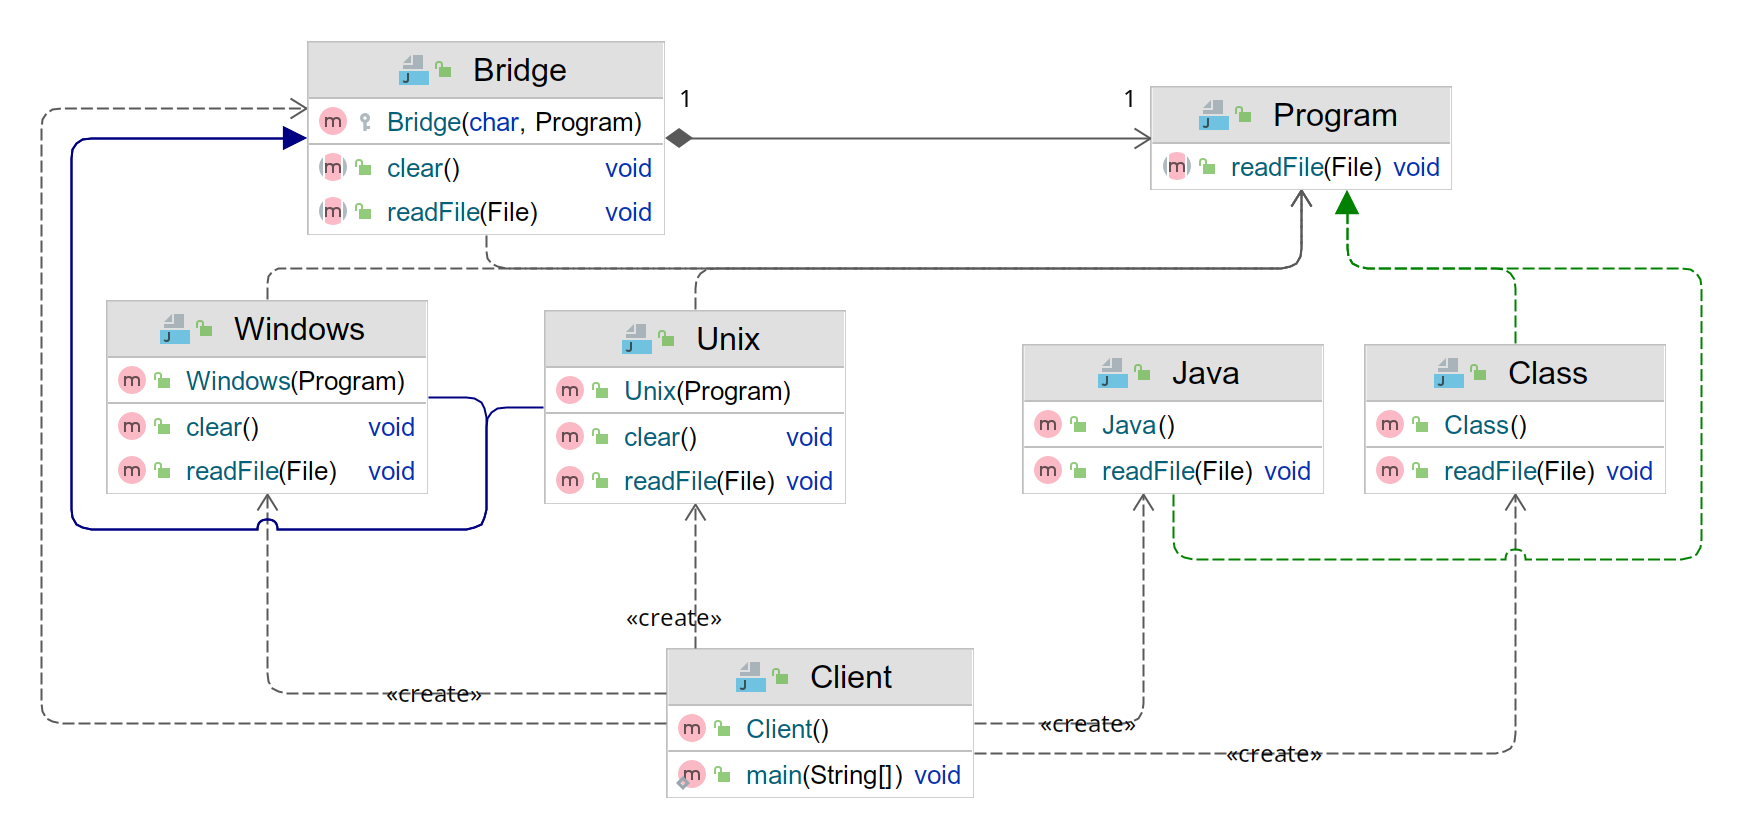
\includegraphics[scale=0.28]{./image/brigde-example.png}
        \end{figure}
        \item[-]\subpara{Chúng ta có một interface là Program làm implementor, 2 class Class và Java kế thừa từ Program. Đại khái chương trình sẽ in nội dung file .class và file .java ra màn hình.}
        \item[-]\subpara{Có một vấn đề là phân cấp đường dẫn trong hai nhóm hệ điều hành Windows và Unix khác nhau, lệnh xóa dữ liệu đã in trên console khác nhau vậy nên ta cần một bridge để có các biến, lệnh tương ứng trên mỗi hệ điều hành. Ở đây abstract class Bridge là Abstraction sẽ có 1 hàm run để gọi hàm của Program, 1 hàm clear để clear console, hằng public final char SEPARATE để lưu dấu phân cấp của OS và 2 class Windows, Unix trong package bridge.os đóng vai trò RefinedAbstraction.}
        \item[-]\subpara{Trong mã nguồn java, giá trị separate này sẽ được hệ điều hành quy định và có thể dùng java.util.Properties getProperty("file.separator") để gọi ra. Abstract class java.io.FileSystem là một Implementor chứa hằng char slash để lưu giá trị này. WinNTFileSystem ở bản jdk Windows và UnixFileSystem ở bản jdk Unix là hai ConcreteImplementor sẽ gọi hàm getProperties để lấy giá trị này. Sau đó java.io.File là Abstraction sẽ lấy tên OS, rồi tạo một đối tượng hằng FileSystem với OS tương ứng, hằng separate gán bằng giá trị slash lấy từ FileSystem. Dưới đây là mô hình đơn giản hóa để lấy dấu phân cấp thư mục:}
        \begin{figure}[htp]
            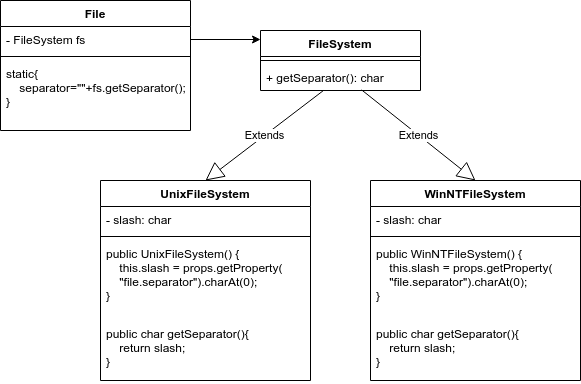
\includegraphics[scale=0.7]{./image/bridge-java.png}
        \end{figure}
        \item[-]\subpara{Ở đây tham số truyền vào của Bridge là dấu phân cấp tương ứng của hệ điều hành và Program. Trong Class của OS dấu phân cấp được quy định sẵn và truyền thêm tham số của Program. Windows hoặc Unix sẽ gọi hàm dựng của super class với 2 đối số là dấu phân cấp và Program. Hàm clear được viết tương ứng với OS và hàm readFile sẽ sẽ gọi đến hàm readFile của Program.}
        \item[-]\subpara{Về phía Client, tạo ra 2 instance Bridge gồm bridgeJava và bridgeClass, lấy tên của OS. Với mỗi OS sẽ tạo ra cặp bridge tương ứng. Qua đó chúng ta có thể dùng hàm trong Bridge để gọi các biến và các hàm trong Program trên hai nhóm OS như code bên dưới.}
        \item[-]\subpara{Trong lúc đóng gói phần mềm, thông thường thì phần mềm chỉ hoạt động trên một nền tảng nhất định, các thư viện thừa của hệ điều hành khác sẽ được loại bỏ.}
    \end{itemize}
    \pagebreak

    \section{Decorator}
    \subsection{Định Nghĩa Và Mô Hình Cấu Trúc}
    \begin{itemize}
        \item[-]\subpara{Decorator Pattern thay đổi một instance riêng lẻ của một class bằng cách tạo một class decorator bao bọc class gốc. Như vậy, việc thay đổi hoặc thêm chức năng của object decorator không ảnh hưởng đến cấu trúc hoặc chức năng của object ban đầu.}
        \item[-]\subpara{Mô hình:}
    \end{itemize}
    \begin{figure}[htp]
        \begin{center}
            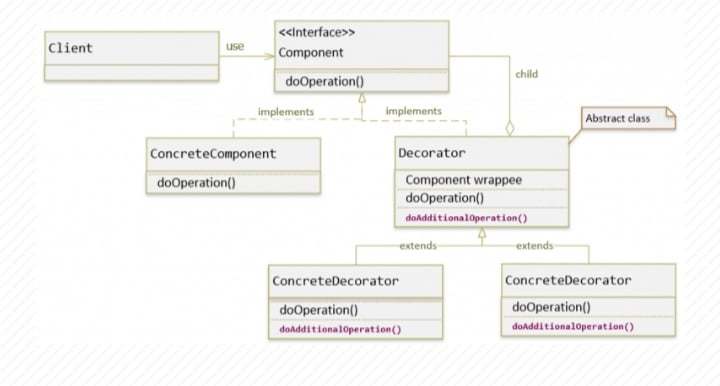
\includegraphics[scale=0.65]{./image/decorator-pattern.jpg}
        \end{center}
    \end{figure}

    \subsection{Đặc điểm}
    \begin{itemize}
        \item[-]\subpara{Có thể bổ sung những chức năng mới cho object}
        \item[-]\subpara{Object gốc không bị thay đổi và cũng không biết gì về những thứ được bổ sung cho nó}
        \item[-]\subpara{Được thực hiện trong thời gian chạy và chỉ áp dụng cho một cá thể}
        \item[-]\subpara{Không cần phải xây dựng class khổng lồ với mọi thứ bên trong}
        \item[-]\subpara{Các object decorator độc lập nhau và có thể tổ hợp với nhau}
    \end{itemize}

    \subsection{Mục Đích Sử Dụng}
    \begin{itemize}
        \item[-]\subpara{Thêm tính năng mới cho đối tượng mà không ảnh hưởng đến các đối tượng}
        \item[-]\subpara{Trong các trường hợp mà việc sử dụng kế thừa sẽ mất nhiều công sức trong việc viết code hoặc không thể mở rộng đối tượng bằng thừa kế}
    \end{itemize}


    \subsection{Code khuôn mẫu}
    \begin{lstlisting}
//Client.java
public class Client {
    public static void main(String[] args) {
        Component component = new ConcreteDecoratorOne(new ConcreteComponent());
        component.doOperation();
        System.out.println("Adding concrete component two...");
        component = new ConcreteDecoratorOne(new ConcreteDecoratorTwo(new ConcreteComponent()));
        component.doOperation();
    }
}

//Component.java
public interface Component {
    public void doOperation();
}

//ConcreteComponent.java
public class ConcreteComponent implements Component {
    @Override
    public void doOperation() {
        System.out.println("Concrete Component doing operation");
    }
}
//Other ConcreteDecorator similar as this
//ConcreteDecorator.java
public class ConcreteDecorator extends Decorator {
    public ConcreteDecorator(Component component) {
        super(component);
    }

    @Override
    public void doOperation() {
        super.doOperation();
        doAdditionalOperation();
    }

    public void doAdditionalOperation() {
        System.out.println("Doing additional operation concrete decorator.");
    }
}

//Decorator.java
public abstract class Decorator implements Component {
    protected Component component;

    public Decorator(Component component){
        this.component = component;
    }

    @Override
    public void doOperation() {
        component.doOperation();
    }
}
    \end{lstlisting}

    \subsection{Giải thích Design Pattern}
    \begin{itemize}
        \item[-]\subpara{Theo Mô hình }
        \begin{itemize}
            \item[+]\subpara{Component: là một interface quy định các method chung cần phải có cho tất cả các thành phần tham gia vào mẫu này.}
            \item[+]\subpara{ConcreteComponent: là lớp hiện thực (implements) các phương thức của Component.}
            \item[+]\subpara{Decorator: là một abstract class dùng để duy trì một tham chiếu của đối tượng Component và đồng thời cài đặt các phương thức của Component interface.}
            \item[+]\subpara{ConcreteDecorator : là lớp hiện thực (implements) các phương thức của Decorator, nó cài đặt thêm các tính năng mới cho Component.}
            \item[+]\subpara{Client : đối tượng sử dụng Component.}
        \end{itemize}
        \item[-]\subpara{Theo code khuôn mẫu}
        \begin{itemize}
            \item[+]\subpara{Component là interface tổng để class ConcreteComponent và abstract class Decorator kế thừa. Tất cả đều có chung 1 hành động là doOperation. ConcreteComponent là một class chứa các hàm sẽ được quy định mặc định như ở đây là doOperation.}
            \item[+]\subpara{Biến thành viên của abstract class Decoration có 1 instance của Component ở trạng thái protected cùng hàm dựng có tham số là Component. Các hàm chung mà các class con của Decoration sẽ sử dụng đều gọi hàm từ instance của Component tức sẽ gọi hàm trong ConcreteComponent. Class con kế thừa từ Decorator là ConcreteDecorator sẽ có hàm dựng với tham số là 1 instance Component và gọi đến hàm khởi tạo của hàm cha qua super. Hàm doOperation của các class con của Decorator có thể thoải mái tùy biến.}
            \item[+]\subpara{Do đã có ConcreteComponent làm chung, Client hoàn toàn có thể khai báo đối tượng kiểu ConcreteComponent hoặc ConcreteDecoration và sau đó có thể chuyển qua lại giữa các ConcreteDecoration.}
        \end{itemize}
    \end{itemize}

    \subsection{Ví Dụ Sử Dụng Trong Thực Tế}
    \begin{itemize}
        \item[-]\subpara{Hệ thống phân quyền sử dụng decorator pattern\\
        \href{https://github.com/blaplafla13th/design-patterns/tree/main/src/decorator}{https://github.com/blaplafla13th/design-patterns/tree/main/src/decorator}}
        \item[-]\subpara{Tạo một interface User đóng vai trò Component với các setter và getter cơ bản các giá trị như PersonalInformation, listAction, hàm để xem (readListAction), thêm (createListAction), sửa (updateListAction), xóa (deleteListAction) (CRUD) ArrayList listAction, hàm thực thi action.}
        \item[-]\subpara{Class SimpleUser đóng vai trò ConcreteComponent với 2 biến thành viên là String PersonalInformation, ArrayList listAction và những chi tiết cho các hàm abstract từ interface.}
        \item[-]\subpara{Abstract class ExtendUser đóng vai trò Decorator để chúng ta có thể mở rộng từ SimpleUser thành SuperUser và NormalUser. Class sẽ compose với interface User, có một biến thành viên là instance của User với kiểu protected để có thể sử dụng ở các hàm mở rộng phía dưới và hàm dựng có tham số là instance của User, hàm dựng không tham số của ExtendUser sẽ tạo mới SimpleUser. Mọi hàm trong ExtendUser kế thừa từ User sẽ được gọi lại thông qua instance user để kế thừa code đã được viết ở SimpleUser. Hai hàm abstract action và resetActionList để các class extend từ class này bắt buộc có.}
        \item[-]\subpara{Hai hàm SuperUser và NormalUser sẽ có các hàm action và resetAction khác nhau. Instance user đang ở protected nên hai hàm con có thể sử dụng thoải mái. Hàm dựng không biến của cả 2 sẽ gọi đến hàm dựng không biến của hàm cha để khởi tạo instance user với mục đích sử dụng resetListAction. Hàm dựng có tham số user và 1 boolean để có thể chuyển đổi kiểu giữa 2 class với boolean để chạy tùy chọn resetActionList. Khi mở rộng thêm các loại User chúng ta chỉ cần tùy biến 2 hàm resetActionList và action.}
        \item[-]\subpara{Ở Client chúng ta có thể sử dụng các hàm được quy định sẵn ở interface User, các hàm dựng. Để chuyển đổi giữa các dạng user chúng ta sử dụng hàm dựng với đối là user cần chuyển.}
        \begin{figure}[htp]
            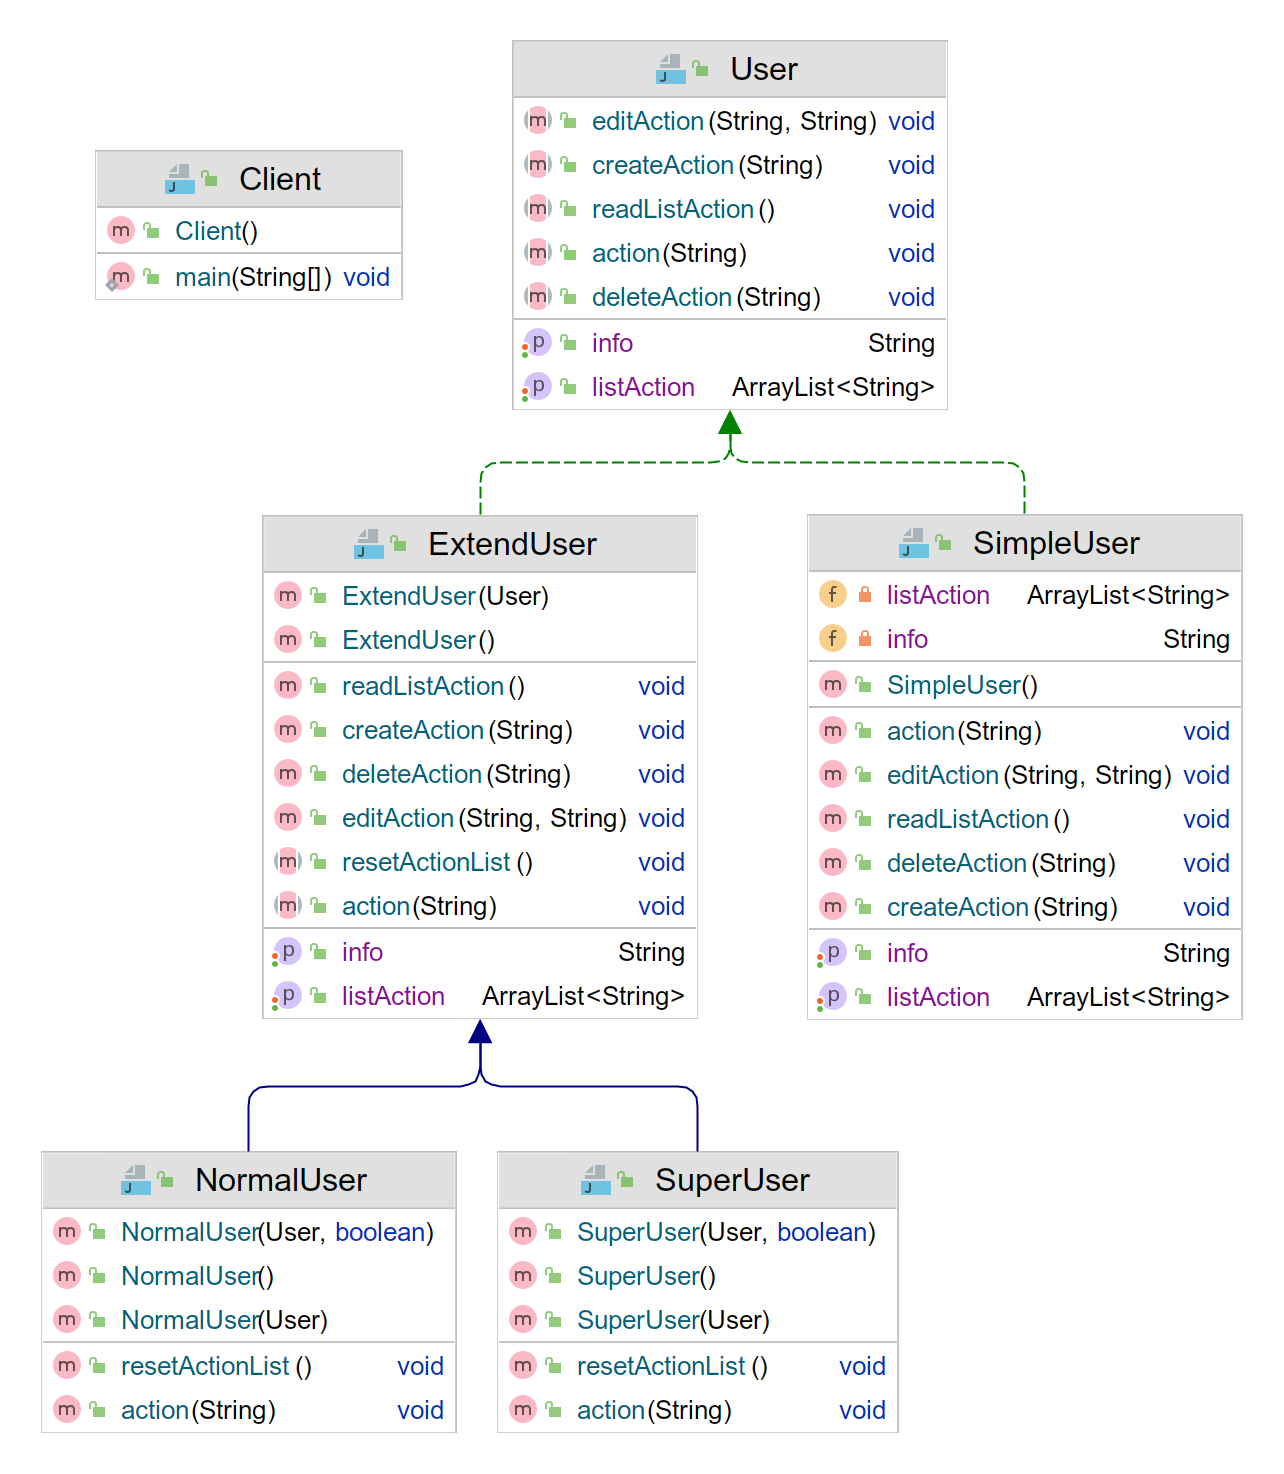
\includegraphics[scale=0.4]{./image/decorator-example.png}
        \end{figure}
    \end{itemize}
    \pagebreak

    \begin{center}
        \hspace{0pt}
        \vfill
        \part{Nhóm hành vi - Behavioral Pattern}
        \begin{figure}[htp]
            \begin{center}
                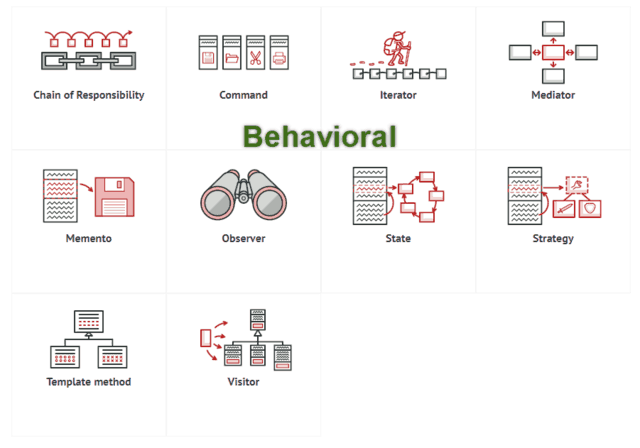
\includegraphics[scale=0.65]{./image/behavioral-pattern.png}
            \end{center}
        \end{figure}
        \vfill
        \hspace{0pt}
    \end{center}
    \pagebreak

    \section{Observer}
    \subsection{Định Nghĩa Và Mô Hình Cấu Trúc}
    \begin{itemize}
        \item[-]\subpara{Observer Pattern định nghĩa mối phụ thuộc một - nhiều giữa các đối tượng để khi mà một đối tượng có sự thay đổi trạng thái, tất cả các thành phần phụ thuộc của nó sẽ được thông báo và cập nhật một cách tự động.}
        \item[-]\subpara{Observer có thể đăng ký với hệ thống. Khi hệ thống có sự thay đổi, hệ thống sẽ thông báo cho Observer biết. Khi không cần nữa, mẫu Observer sẽ được gỡ khỏi hệ thống.}
        \item[-]\subpara{Mô hình:}
    \end{itemize}
    \begin{figure}[htp]
        \begin{center}
            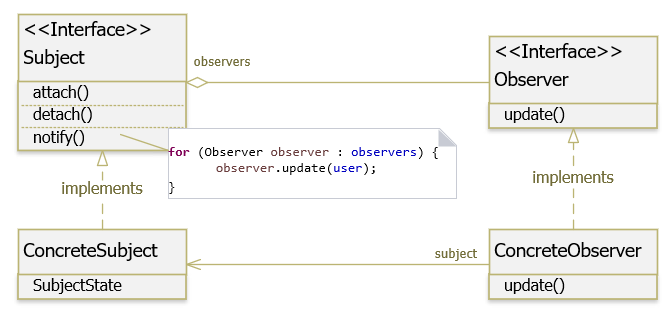
\includegraphics[scale=0.65]{./image/observer-pattern.png}
        \end{center}
    \end{figure}

    \subsection{Đặc điểm}
    \begin{itemize}
        \item[-]\subpara{Cho phép thay đổi Subject và Observer một cách độc lập, có thể tái sử dụng các Subject mà không cần tái sử dụng các Observer và ngược lại}
        \item[-]\subpara{Cho phép thêm Observer mà không sửa đổi Subject hoặc Observer khác}
        \item[-]\subpara{Một đối tượng có thể thông báo đến một số lượng không giới hạn các đối tượng khác}
    \end{itemize}

    \subsection{Mục Đích Sử Dụng}
    \begin{itemize}
        \item[-]\subpara{Thường được sử dụng trong mối quan hệ một - nhiều giữa các object với nhau. Trong đó, một đối tượng thay đổi và muốn thông báo cho tất cả các object liên quan biết về sự thay đổi đó}
        \item[-]\subpara{Sử dụng trong ứng dụng broadcast - type communication}
        \item[-]\subpara{Sử dụng để quản lý sự kiện (Event management)}
        \item[-]\subpara{Sử dụng trong mẫu mô hình MVC (Model View Controller Pattern)}
    \end{itemize}

    \subsection{Code khuôn mẫu}
    \begin{lstlisting}
//Observer.java
public interface Observer {
    void update();
}

//Subject.java
public interface SubjectA {
    public void add(Observer o);

    public int getState();

    public void setState(int value);

    private void execute();
}

//SubjectA.java
public class SubjectA implements Subject{
    private List<Observer> observers = new ArrayList<>();
    private int state;

    public void add(Observer o) {
        observers.add(o);
    }

    public int getState() {
        return state;
    }

    public void setState(int value) {
        this.state = value;
        execute();
    }

    private void execute() {
        for (Observer observer : observers) {
            observer.update();
        }
    }
}

//SubjectB,C similar as SubjectA

//ObserverA.java
public class ObserverA implements Observer {
    protected Subject subject;
    public ObserverA(Subject subject) {
        this.subject = subject;
        this.subject.add(this);
    }

    public void update() {
        ...
    }
}

//ObserverB,C similar as ObserverA

    \end{lstlisting}

    \subsection{Giải thích Design Pattern}
    \begin{itemize}
        \item[-]\subpara{Theo Mô hình }
        \begin{itemize}
            \item[+]\subpara{Subject: chứa danh sách các observer, cung cấp phương thức để có thể thêm và loại bỏ observer.}
            \item[+]\subpara{Observer: định nghĩa một phương thức update() cho các đối tượng sẽ được subject thông báo đến khi có sự thay đổi trạng thái.}
            \item[+]\subpara{ConcreteSubject: cài đặt các phương thức của Subject, lưu trữ trạng thái danh sách các ConcreateObserver, gửi thông báo đến các observer của nó khi có sự thay đổi trạng thái.}
            \item[+]\subpara{ConcreteObserver: cài đặt các phương thức của Observer, lưu trữ trạng thái của subject, thực thi việc cập nhật để giữ cho trạng thái đồng nhất với subject gửi thông báo đến.}
        \end{itemize}
        \item[-]\subpara{Theo code khuôn mẫu}
        \begin{itemize}
            \item[+]\subpara{Subject: cung cấp phương thức để có thể thêm observer, lấy giá trị, đặt giá trị cho observer và đồng bộ các observer. SubjectA, B... có ArrayList các observer sẽ đồng bộ và state là dữ liệu lưu trữ trạng thái danh sách mà observer sẽ đồng bộ. Các phương thức kế thừa ở trên như add để thêm, getState để lấy giá trị, setState để đặt giá trị và execute để gọi tất cả các phần tử update. Nếu như SubjectA, B... giống nhau chúng ta có thể để Subject là abstract class để extend, thậm chí giống hệt nhau thì chỉ cần để mỗi class Subject để tái sử dụng tối đa code.}
            \item[+]\subpara{Observer: định nghĩa một phương thức update() cho các đối tượng sẽ được subject thông báo đến khi có sự thay đổi trạng thái. ObserverA, B implements từ observer có hàm dựng với tham số bắt buộc là Subject để khi làm việc các object sẽ có chung 1 đối tượng thực hiện ra lệnh update trạng thái. Và tương tự với Subject có thể rút gọn code bằng cách sử dụng abstract class hoặc class.}

        \end{itemize}
    \end{itemize}

    \subsection{Ví Dụ Sử Dụng Trong Thực Tế}
    \begin{itemize}
        \item[-]\subpara{Hệ thống chat đơn giản sử dụng Observer pattern\\
        https://github.com/blaplafla13th/design-patterns/tree/main/src/observer}
        \begin{figure}[htp]
            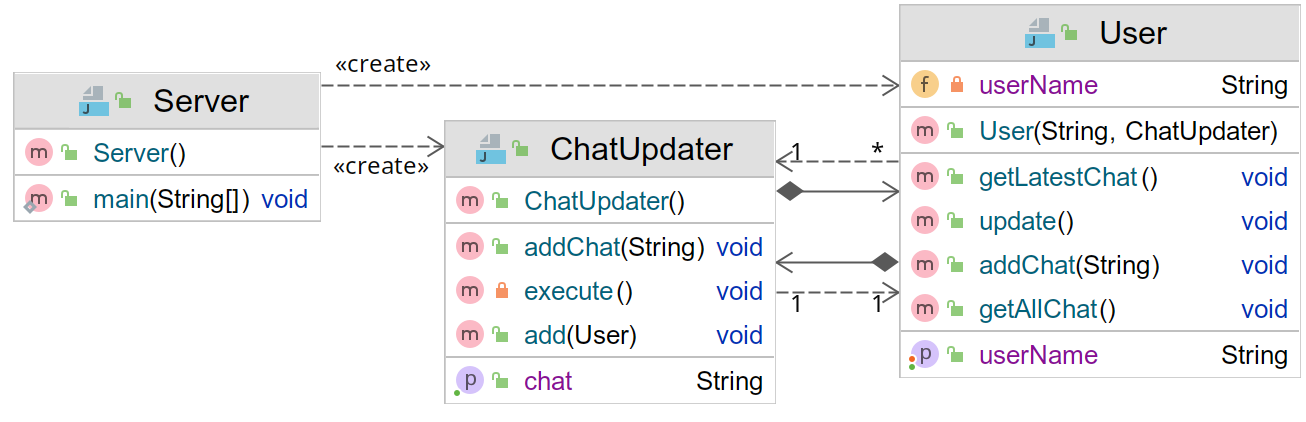
\includegraphics[scale=0.5]{./image/observer-example.png}
        \end{figure}
        \item[-]\subpara{Thay vì dùng Interface, để đơn giản và tái sử dụng được nhiều code ta sử dụng class. Ở đây, User đóng vai trò vừa là Subject vừa là Concrete Subject. Observer và Concrete sẽ là ChatUpdater. Server đóng vai trò giao tiếp với người dùng. Trong ứng dụng thực tế thì ngoài 3 class trên, do user ở 2 máy khác nhau nên cần 1 class để chuyển dữ liệu qua lại bằng socket qua mạng và các tin nhắn được lưu trên file riêng. Code này để chạy thử nên tạo 2 instance của User là user1,2 làm Observer và có thể tự chat giữa hai user.}
        \item[-]\subpara{ChatUpdater sẽ có 1 ArrayList<User> user để lưu list các người dùng tham gia luồng chat này. String message để lưu tin nhắn cuối cùng nhận được. Hàm add với tham số là User sẽ thêm user vào ArrayList users. Trong hàm add có 1 lệnh users.add(user) để thêm user và 1 lệnh addChat để thông báo có user mới tham gia. Hàm getChat sẽ trả về message còn hàm addChat với tham số truyền vào là String sẽ cập nhật message và chạy hàm execute. Trong hàm execute, 1 vòng for để gọi mọi User trong user chạy hàm update.}
        \item[-]\subpara{User có biến thành viên String userName để lưu tên người dùng, ChatUpdater để có luồng chat nhận/gửi thông tin và ArrayList<String> listMessage để lưu các tin nhắn đã nhận. Thêm các hàm như hàm update để nhận dữ liệu từ hàm getChat() ở ChatUpdater cho vào listMessage, hàm getAllChat để in ra tất cả chat đã lưu, getLatestChat để in tin nhắn cuối cùng nhận được và hàm addChat sẽ gọi ChatUpdater ở phía trên, sau đó ChatUpdater gọi đến hàm addChat để gửi tin nhắn. Thêm 2 hàm để xem và sửa tên người dùng. Hàm dựng sẽ gồm 2 tham số là userName và ChatUpdater, trong hàm dựng sẽ thêm lệnh chatUpdater(this) để thêm người dùng vào luồng chat.}
        \item[-]\subpara{Tiếp theo đến Server, chúng ta tạo một chatUpdater để tên là chatThread. Tạo mới User tên user1 với 2 đối số là user với giá trị là "Blaplafla" và chatUpdater là chatThread. Khi chạy user1.getLatestChat sẽ nhận được câu chào của chatUpdater khi thêm user mới, tương tự với user2. Dùng chatThread.addChat để xem đồng bộ giữa 2 user. Khi getAllMessage, user1 sẽ có 3 tin là chào user1, chào user2, và chào mừng đến với server còn user2 do được thêm vào sau user1 nên không có tin chào user1 tức toàn bộ tin nhắn phía trước. Sau đó chúng ta chat thử, dùng user1.addChat và xem toàn bộ tin nhắn của user2 sẽ thấy tin nhắn của user1 ở dưới.}
    \end{itemize}
    \pagebreak

    \section{Iterator}
    \subsection{Định Nghĩa Và Mô Hình Cấu Trúc}
    \begin{itemize}
        \item[-]\subpara{Iterator Pattern cho phép xử lý nhiều loại tập hợp khác nhau bằng cách truy cập từng phần tử của tập hợp với cùng một phương pháp, cùng một cách thức định sẵn mà không cần phải hiểu rõ về những chi tiết bên trong những tập hợp này.}
        \item[-]\subpara{Iterator thường được viết trong Java như là những lớp độc lập - một lớp chỉ có duy nhất một công việc để làm.}
        \item[-]\subpara{Mô hình:}
    \end{itemize}
    \begin{figure}[htp]
        \begin{center}
            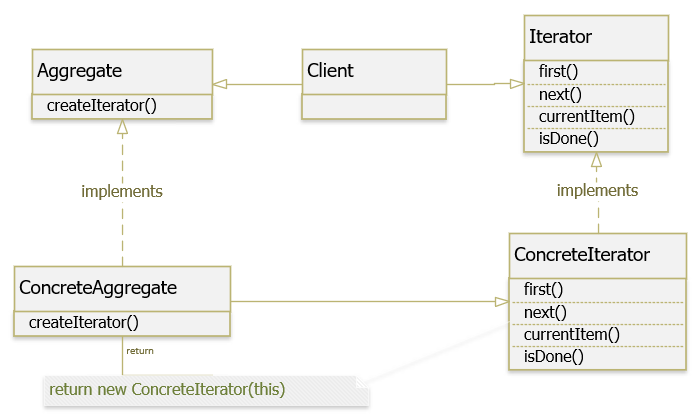
\includegraphics[scale=0.65]{./image/iterator-pattern.png}
        \end{center}
    \end{figure}

    \subsection{Đặc điểm}
    \begin{itemize}
        \item[-]\subpara{Tách phần cài đặt các phương thức của tập hợp (collection) và phần duyệt qua các phần tử (iterator) theo từng class riêng lẻ}
        \item[-]\subpara{Có thể implement các loại collection mới và iterator mới, sau đó chuyển chúng vào code hiện có}
        \item[-]\subpara{Có thể truy cập song song trên cùng một collection vì mỗi đối tượng iterator có chứa trạng thái riêng của nó}
    \end{itemize}

    \subsection{Mục Đích Sử Dụng}
    \begin{itemize}
        \item[-]\subpara{Truy cập nội dung của đối tượng trong tập hợp mà không cần biết nội dung cài đặt bên trong}
        \item[-]\subpara{Hỗ trợ truy xuất nhiều loại tập hợp khác nhau}
        \item[-]\subpara{Cung cấp một interface duy nhất, đơn giản, nhất quán để làm việc với các tập hợp khác nhau}
    \end{itemize}

    \subsection{Code khuôn mẫu}
    \begin{lstlisting}
//Iterator.java
public interface Iterator {
    public boolean hasNext();
    public Object next();
}

//Aggregate.java
public interface Aggregate {
    public Iterator getIterator();
}

//ConcreteAggregate.java
public class ConcreteAggregate implements Aggregate {
    public String[] collections=...;

    @Override
    public Iterator getIterator() {
        return new ConcreteIterator(this) ;
    }

    //ConcreteIterator
    private class ConcreteIterator implements Iterator {
        int i;
        @Override
        public boolean hasNext() {
            if (i < collections.length) {
                return true;
            }
            return false;
        }

        @Override
        public Object next() {
            if (this.hasNext()) {
                return collections[i++];
        }
            return null;
        }
    }
}
    \end{lstlisting}

    \subsection{Giải thích Design Pattern}
    \begin{itemize}
        \item[-]\subpara{Theo Mô hình }
        \begin{itemize}
            \item[+]\subpara{Aggregate: là một interface định nghĩa định nghĩa các phương thức để tạo Iterator object.}
            \item[+]\subpara{ConcreteAggregate: cài đặt các phương thức của Aggregate, nó cài đặt một interface tạo Iterator để trả về một thể hiện của ConcreteIterator thích hợp.}
            \item[+]\subpara{Iterator: là một interface hay abstract class, định nghĩa các phương thức để truy cập và duyệt qua các phần tử.}
            \item[+]\subpara{ConcreteIterator: cài đặt các phương thức của Iterator, giữ index khi duyệt qua các phần tử.}
            \item[+]\subpara{Client: đối tượng sử dụng Iterator Pattern, nó yêu cầu một iterator từ một đối tượng collection để duyệt qua các phần tử mà nó giữ. Các phương thức của iterator được sử dụng để truy xuất các phần tử từ collection theo một trình tự thích hợp.}
        \end{itemize}
        \item[-]\subpara{Theo code khuôn mẫu}
        \begin{itemize}
            \item[+]\subpara{Trong Interface Iterator chứa 2 phương thức hasNext kiểm tra có phhần tử tiếp theo không và next để trả về phần tử tiếp theo. ConcreteIterator implement từ Iterator là 1 private class nằm trong ConcreteAggregate chứa thêm biến thành viên int i để counter.}
            \item[+]\subpara{ConcreteAggregate: cài đặt các phương thức của Aggregate, nó cài đặt một interface tạo Iterator để trả về một thể hiện của ConcreteIterator thích hợp.}
            \item[+]\subpara{Aggregate là interface có 1 hàm trả về Iterator object, ConcreteAggregate kế thừa từ hàm này chứa 1 mảng String và 1 hàm trả về ConcreteIterator của chính nó.}
        \end{itemize}
    \end{itemize}

    \subsection{Ví Dụ Sử Dụng Trong Thực Tế}
    \begin{itemize}
        \item[-]\subpara{Có thể nói Iterator là 1 trong những design pattern phổ biến nhất. Điển hình như ArrayList. Trong Java, Iterator là java.utils.Iterator, ArrayList là 1 ConcreteAggregate, rất nhiều class private class trong ArrayList là ConcreteIterator. Do được sử dụng quá nhiều, nhà phát triển java đã sử dụng generic để tối ưu thuận tiện nhất cho người sử dụng.}
        \item[-]\subpara{Mô hình minh họa sơ lược về Iterator và Arraylist trong java:}
        \begin{figure}[htp]
            \begin{center}
                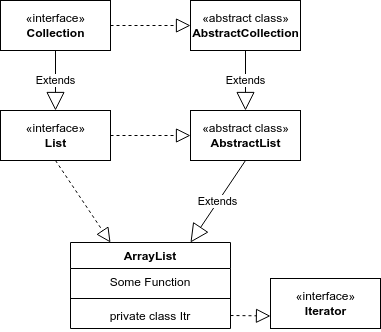
\includegraphics[scale=0.8]{./image/iterator-java.png}
            \end{center}
        \end{figure}
        \item[-]\subpara{Ví dụ Bookmark sử dụng Iterator \\ \href{https://github.com/blaplafla13th/design-patterns/tree/main/src/iterator}{https://github.com/blaplafla13th/design-patterns/tree/main/src/iterator}}
        \begin{figure}[htp]
            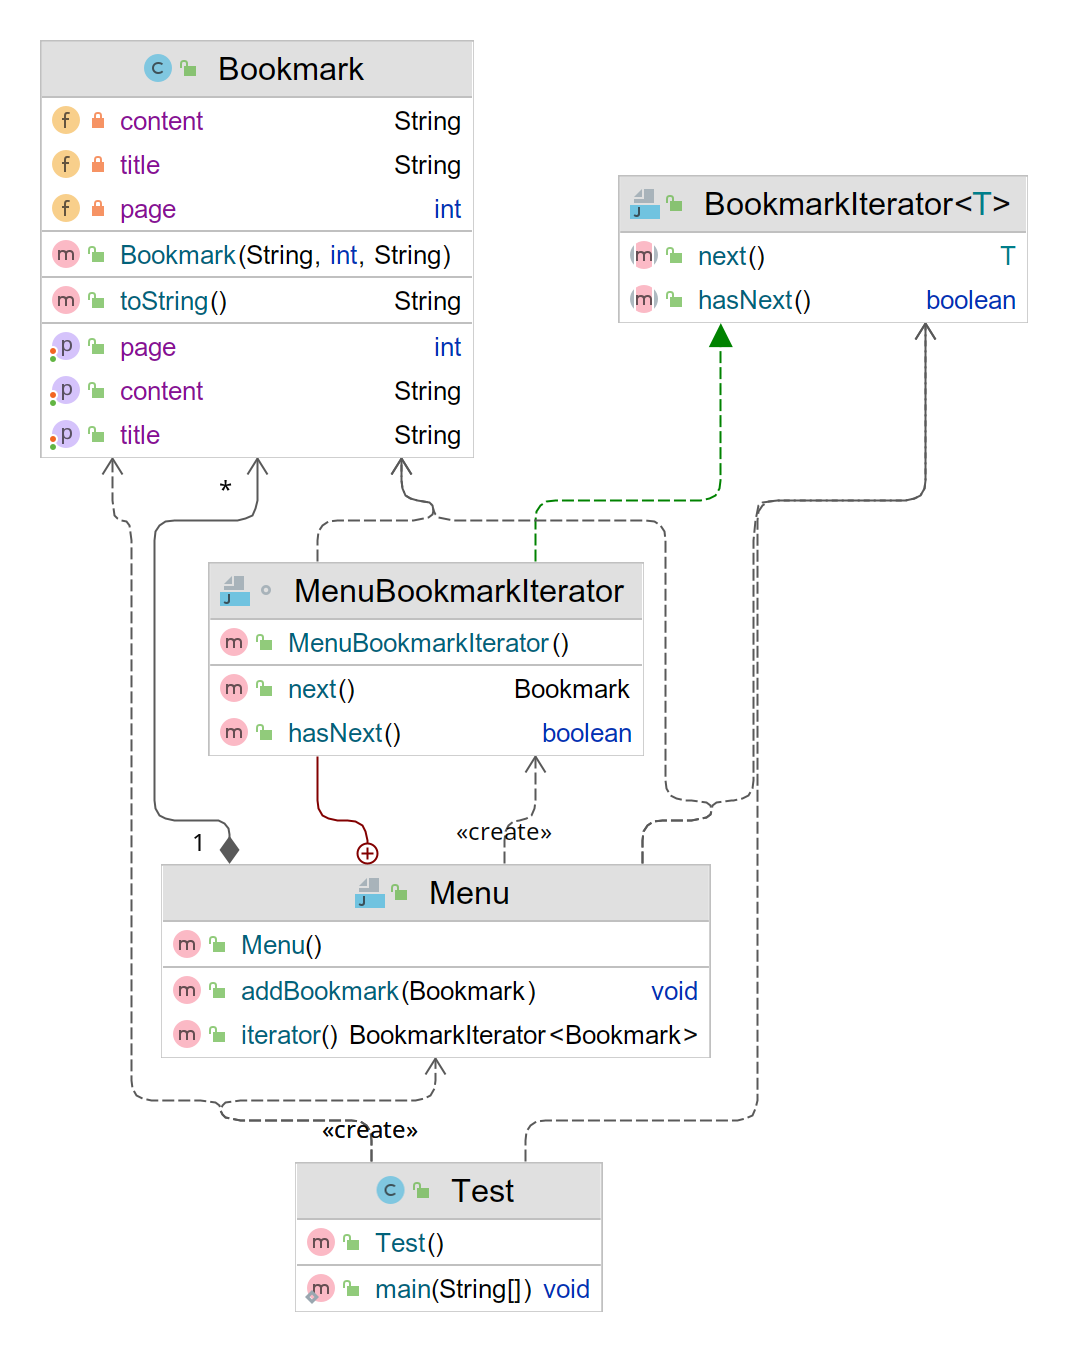
\includegraphics[scale=0.33]{./image/iterator-example.png}
        \end{figure}
        \item[-]\subpara{Class Bookmark chứa 3 biến thành viên, hàm dựng đủ 3 tham số cũng như getter, setter, toString làm object chạy thử.}
        \item[-]\subpara{Interface BookmarkIterator đóng vai trò Interator, có tác dụng như đã nói ở trên.}
        \item[-]\subpara{Lớp Menu chứa 1 arraylist để lưu bookmark, một hàm thêm phần tử vào arraylist và một hàm trả về instance của class MenuBookmarkIterator mở rộng từ BookmarkIterator. Trong MenuBookmarkIterator gồm 1 biến thành viên currentIndex để lưu indêx và 2 hàm next và hasNext.}
    \end{itemize}
    \pagebreak

    \section{Command}
    \subsection{Định Nghĩa Và Mô Hình Cấu Trúc}
    \begin{itemize}
        \item[-]\subpara{Command Pattern chuyển yêu cầu thành đối tượng độc lập, có thể được sử dụng để tham số hóa các đối tượng với các yêu cầu khác nhau. Nói cách khác, nó cho phép tất cả những request gửi đến object được lưu trữ trong chính object đó dưới dạng một object command (một class trung gian lưu trữ các câu lệnh và trạng thái của object tại một thời điểm nào đó).}
        \item[-]\subpara{Mô hình:}
    \end{itemize}
    \begin{figure}[htp]
        \begin{center}
            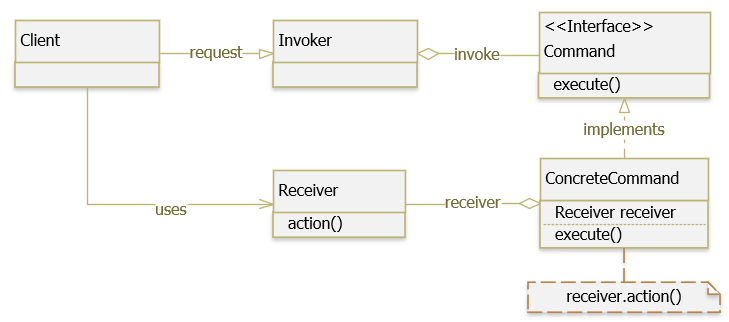
\includegraphics[scale=0.6]{./image/command-pattern.png}
        \end{center}
    \end{figure}

    \subsection{Đặc điểm}
    \begin{itemize}
        \item[-]\subpara{Chia nhỏ chương trình thành các module Command nên dễ dàng thêm các Command mới trong hệ thống mà không cần thay đổi trong các lớp hiện có, khi một trong những class Command bị lỗi không gây lỗi cho toàn hệ thống}
        \item[-]\subpara{Tách đối tượng gọi operation từ đối tượng thực sự thực hiện operation. Giảm kết nối giữa Invoker và Receiver}
        \item[-]\subpara{Dễ dàng chuyển dữ liệu dưới dạng đối tượng giữa các thành phần hệ thống}
        \item[-]\subpara{Tăng số lớp cho từng lệnh riêng lẻ}
    \end{itemize}

    \subsection{Mục Đích Sử Dụng}
    \begin{itemize}
        \item[-]\subpara{Khi cần tham số hóa các đối tượng theo một hành động thực hiện}
        \item[-]\subpara{Tạo và thực thi các yêu cầu vào các thời điểm khác nhau}
        \item[-]\subpara{Khi cần hỗ trợ tính năng như undo, log, callback hoặc transaction, ...}
    \end{itemize}

    \subsection{Code khuôn mẫu}
    \begin{lstlisting}
//Receiver.java
public class Receiver {
    ...
    public void action(){
        ...
    }
}

//Command.java
public abstract class Command {
    public abstract void execute();
}

//ConcreteCommandA.java
public class ConcreteCommandA extends Command {
    private Receiver receiver;

    @Override
    public void execute() {
        ...
        receiver.action();
        ...
    }
}
//ConcreteCommandB,C... similar as  ConcreteCommandA

//Invoker.java
public class Invoker {
    Command command;
    public Invoker(Command command){
        ...
    }
    public void action(){
        ...
        command.execute();
        ...
    }
}

//Client.java
public class Client {
    public static void main(String[] args) {
        Invoker invoker=new Invoker(new ConcreteCommandA(new Receiver()));
        ...
    }
}
    \end{lstlisting}

    \subsection{Giải thích Design Pattern}
    \begin{itemize}
        \item[-]\subpara{Theo Mô hình }
        \begin{itemize}
            \item[+]\subpara{Command: là một interface hoặc abstract class, chứa một phương thức trừu tượng thực thi (execute), một hành động (operation). Request sẽ được đóng gói dưới dạng Command.}
            \item[+]\subpara{ConcreteCommand: là các implementation của Command. Định nghĩa một sự gắn kết giữa một đối tượng Receiver và một hành động. Thực thi execute() bằng việc gọi operation đang hoãn trên Receiver. Mỗi một ConcreteCommand sẽ phục vụ cho một case request riêng gọi là module.}
            \item[+]\subpara{Client: tiếp nhận request từ phía người dùng, đóng gói request thành ConcreteCommand thích hợp và thiết lập receiver của nó.}
            \item[+]\subpara{Invoker: tiếp nhận các module là ConcreteCommand từ Client và gọi execute() của ConcreteCommand để thực thi request.}
            \item[+]\subpara{Receiver: đây là thành phần thực sự xử lý business logic cho case request. Trong phương thức execute() của ConcreteCommand chúng ta sẽ gọi method thích hợp trong Receiver.}
        \end{itemize}
        \item[-]\subpara{Theo code khuôn mẫu}
        \begin{itemize}
            \item[+]\subpara{Receiver là class chúng ta sẽ dùng hàm execute ConcreteCommand để sử dụng hàm action một cách hợp lý.}
            \item[+]\subpara{ConcreteCommandA, B...: là các implementation của Command. Tất cả đều theo khuôn mẫu của class Command có hàm execute, như đã nói ở trên execute sẽ gọi hàm action của Receiver.}
            \item[+]\subpara{Client: tạo các đối tượng  Receiver, Command, Invoke và ra lệnh cho Invoker thực hiện các command thao tác với receiver.}
            \item[+]\subpara{Invoker: tiếp nhận các module là ConcreteCommand từ Client và gọi execute() của ConcreteCommand để thực thi yêu cầu từ client.}
        \end{itemize}
    \end{itemize}

    \subsection{Ví Dụ Sử Dụng Trong Thực Tế}
    \begin{itemize}
        \item[-]\subpara{Phần mềm quản lý file sử dụng Command pattern \\
        \href{https://github.com/blaplafla13th/design-patterns/tree/main/src/command}{https://github.com/blaplafla13th/design-patterns/tree/main/src/command}}
        \begin{figure}[htp]
            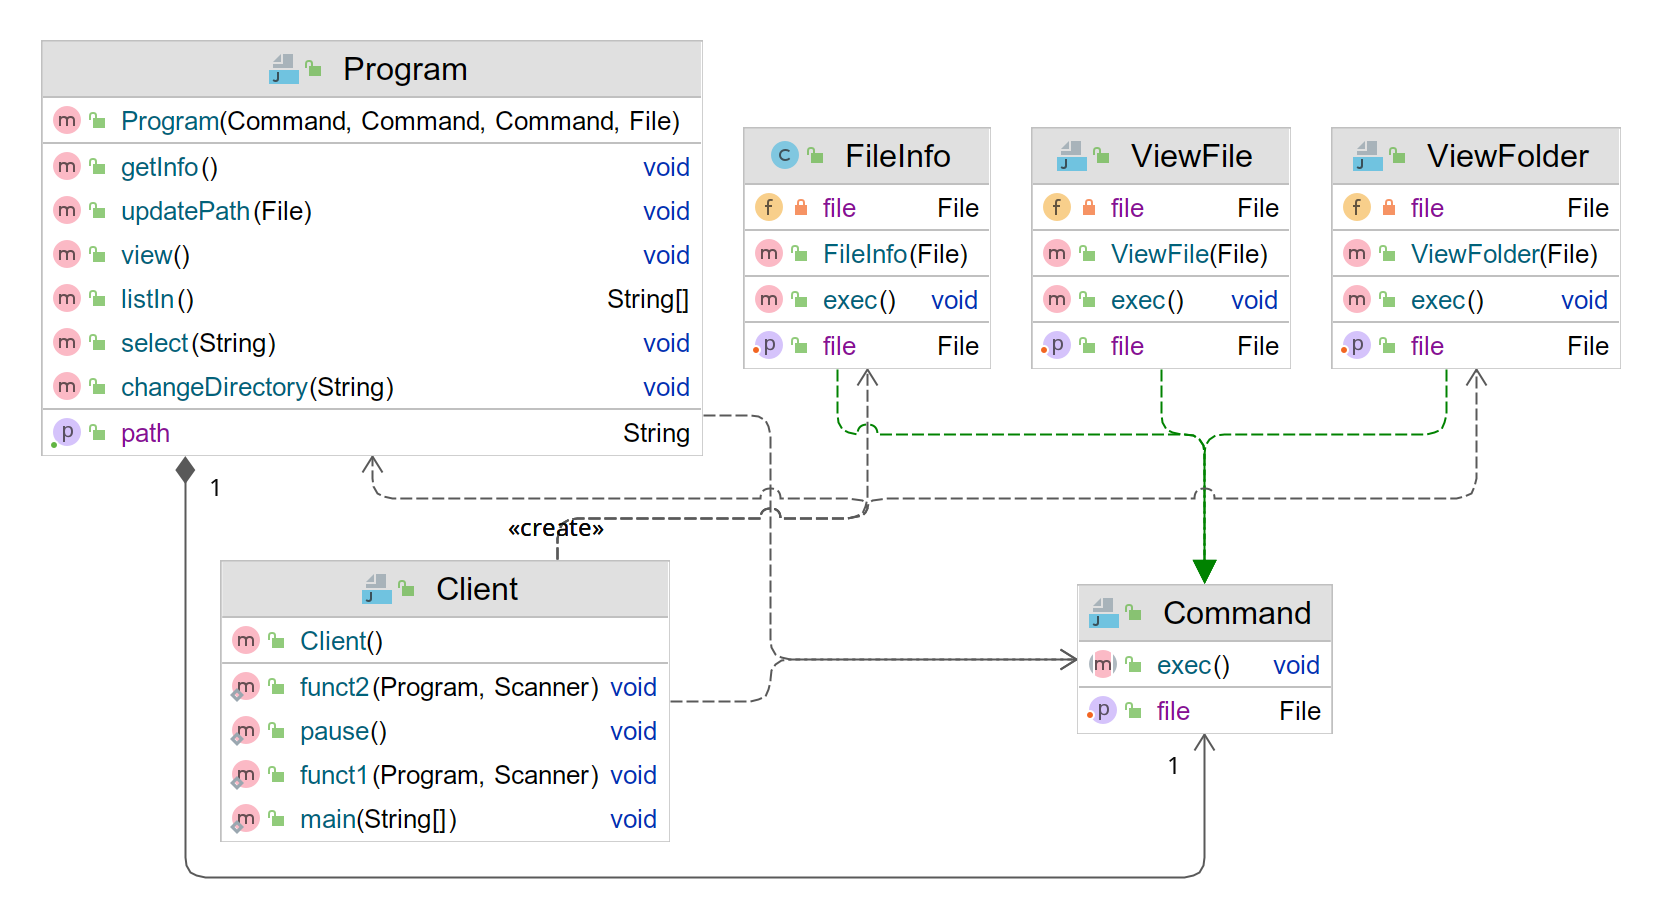
\includegraphics[scale=0.27]{./image/command-example.png}
        \end{figure}
        \item[-]\subpara{Do đây là phần mềm quản lý File nên java.io.File đóng vai trò là 1 Receiver. Invoker nhận request từ Client là Program. ConcreteCommand bao gồm các file FileInfo, ViewFile, ViewFolder.}
        \item[-]\subpara{Invoker gồm các biến thành viên là class con của Command và 1 biến là File. Do 3 class con đều có biến thành viên là file nên cần hàm update với tham số là file để đồng bộ giữa các class tránh trường hợp mỗi class dùng 1 file. THêm một hàm dựng đủ các tham số cho các biến con. Hàm changeDirectory để đổi đường dẫn thành đường dẫn nhập vào, hàm select để đổi sang đường dẫn con của thư mục. Cả hai phương thức đều có cùng tham số đầu vào là String path tạo File tmpfile mới, kiểm tra tính tồn tại (nếu không sẽ dừng còn nếu có sẽ chạy hàm update để cập nhật). Hàm view sẽ kiểm tra xem file hay folder để gọi object tương ứng, getInfo gọi instance của FileInfo, cả 2 đều gọi hàm exec từ Interface Command để chạy. Hàm getPath trả về đường dẫn của file gọi từ Class file, hàm listIn trả về list các files trong folder. hai hàm này chưa tách biệt thành module như 3 file con implement từ Command.}
        \item[-]\subpara{Class con implement từ Interface Command đều có 1 biến thành viên là File files, hàm khởi tạo với tham số là file, hàm setFile. Hàm exec ở ViewFile có nhiệm vụ in ra nội dung File còn với ViewFolder là in ra các file bên trong folder và FileInfo là in ra thông tin cơ bản của file. Tất cả đều có try catch để khi không tìm thấy file sẽ báo lỗi.}
        \item[-]\subpara{Phía Client, chúng ta tạo một chương trình chạy thử. Tạo 6 biến đối tượng Scanner để nhập, File với tham số đường dẫn là hiện tại, 3 class con của Command với tham số là file ở trên cùng, Program với 4 tham số là file và 3 command ở trên. Tiếp theo là 1 vòng while vô tận. Đầu tiên sẽ xóa màn hình, in ra các lựa chọn, nhập lựa chọn, xóa màn hình và xử lý lựa chọn.}
        \item[-]\subpara{Option thứ nhất chưa tách nhưng vẫn khá đơn giản, phần xử lý logic nằm trọn trong class Program. Option thứ 2 chưa được tách thành module riêng nên phần xử lý logic xuất hiện ở cả class Client lẫn class Program. Option thứ 3 thì phần xử lý logic nằm ở các class con của Command và Program chỉ có nhiệm vụ chọn Stragety tương ứng, không bị lộ ở Client. Còn ở option thứ 4 phần logic nằm ở Class ViewInfo. Như vậy, ta thấy việc tách thành từng module như design pattern Command lợi như thế nào. Nếu như 1 tính năng bị lỗi, các tính năng khác vẫn hoạt động. Nhưng nếu như option thứ 2 mà bị lỗi có khả năng rất lớn sẽ lỗi cả chương trình do liên quan đến class Client và class quản lý các module Program.}
    \end{itemize}
    \pagebreak

    \section{Strategy}

    \subsection{Định Nghĩa Và Mô Hình Cấu Trúc}
    \begin{itemize}
        \item[-]\subpara{Strategy Pattern định nghĩa tập hợp các thuật toán, đóng gói từng thuật toán lại và dễ dàng thay đổi linh hoạt các thuật toán bên trong object. Strategy cho phép thuật toán biến đổi độc lập khi người dùng sử dụng chúng.}
        \item[-]\subpara{Cụ thể và dễ hiểu hơn, Strategy Pattern tách rời phần xử lý một chức năng cụ thể ra khỏi đối tượng. Sau đó tạo ra một tập hợp các thuật toán để xử lý chức năng đó và lựa chọn thuật toán nào mà chúng ta thấy đúng đắn nhất khi thực thi chương trình.}
    \end{itemize}
    \begin{figure}[htp]
        \begin{center}
            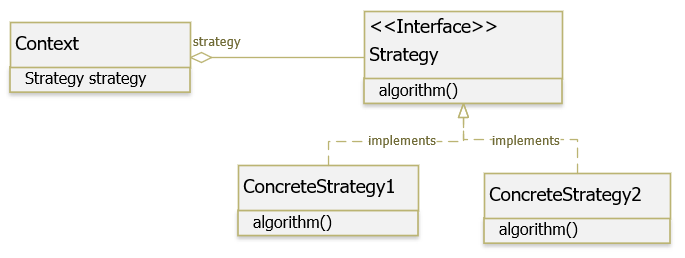
\includegraphics[scale=0.65]{./image/strategy-pattern.png}
        \end{center}
    \end{figure}

    \subsection{Đặc điểm}
    \begin{itemize}
        \item[-]\subpara{Strategy Pattern là một mô hình khởi tạo một lần, không có sự luân chuyển trạng thái}
        \item[-]\subpara{Bất kỳ loại trạng thái nào cũng có thể được khởi tạo một cách độc lập, chúng không biết được sự tồn tại của các Strategy khác}
        \item[-]\subpara{Dễ dàng mở rộng và kết hợp hành vi mới mà không thay đổi ứng dụng}
    \end{itemize}

    \subsection{Mục Đích Sử Dụng}
    \begin{itemize}
        \item[-]\subpara{Muốn thay đổi các thuật toán được sử dụng bên trong một đối tượng tại thời điểm run-time}
        \item[-]\subpara{Bảo trì những đoạn code dễ thay đổi}
        \item[-]\subpara{Tránh sự rắc rối, khi phải hiện thực một chức năng nào đó qua quá nhiều lớp con}
        \item[-]\subpara{Che giấu sự phức tạp, cấu trúc bên trong của thuật toán}
    \end{itemize}

    \subsection{Code khuôn mẫu}
    \begin{lstlisting}
//Strategy.java
public interface Strategy {
    public String doSomething();
}

//ConcreteStrategyA.java
public class ConcreteStrategyA implements Strategy {
    @Override
    public String doSomething() {
        return "ConcreteStrategyA";
    }
}

//ConcreteStrategyB,C,... similar as ConcreteStrategyA

//Context.java
public class Context {
    private Strategy strategy;

    public Context() {
    ...
    }

    public void setStrategy(Strategy behavior) {
        this.strategy = behavior;
    }

    public Strategy getStrategy() {
        return strategy;
    }

    public void executeStrategy(){
        System.out.println(strategy.doSomething());
    }
}
    \end{lstlisting}

    \subsection{Giải thích Design Pattern}
    \begin{itemize}
        \item[-]\subpara{Theo Mô hình }
        \begin{itemize}
            \item[+]\subpara{Strategy: định nghĩa các hành vi có thể có của một Strategy.}
            \item[+]\subpara{ConcreteStrategy: cài đặt các hành vi cụ thể của Strategy.}
            \item[+]\subpara{Context: chứa 1 tham chiếu đến đối tượng Strategy và nhận các yêu cầu từ Client, các yêu cầu này sau đó được ủy quyền cho Strategy thực hiện.}
        \end{itemize}
        \item[-]\subpara{Theo code khuôn mẫu}
        \begin{itemize}
            \item[+]\subpara{Interface Strategy chứa hàm doSomething để các ConcreteStrategy cài đặt sử dụng.}
            \item[+]\subpara{Context: chứa một tham chiếu đến đối tượng Strategy và hàm dựng không đối, getter và setter để chọn đối tượng trong các ConcreteStrategy. Hàm executeStrategy sẽ có nhiệm vụ sau chạy hàm doSomething ở Strategy từ object ConcreteStrategy đã được chỉ định.}
        \end{itemize}
    \end{itemize}

    \subsection{Ví Dụ Sử Dụng Trong Thực Tế}
    \begin{itemize}
        \item[-]\subpara{Quay lại với ví dụ hệ thống thanh toán đơn giản sử dụng factory pattern\\
        \href{https://github.com/blaplafla13th/design-patterns/tree/main/src/factory}{https://github.com/blaplafla13th/design-patterns/tree/main/src/factory}}
        \item[-]\subpara{Strategy pattern thường được kết hợp với Factory pattern khi mà Factory pattern sẽ tạo ra đối tượng (nên thuộc nhóm Creational), Strategy pattern sẽ quyết định hành vi của các hàm trong đối tượng (nên thuộc nhóm Behavioral) và cũng khác đôi chút là Context Stragety sẽ làm thêm nhiệm vụ gọi hàm so với Factory.}
        \item[-]\subpara{Giờ là ví dụ hệ thống thanh toán đơn giản sử dụng stragety pattern\\
        \href{https://github.com/blaplafla13th/design-patterns/tree/main/src/stragety}{https://github.com/blaplafla13th/design-patterns/tree/main/src/stragety}}
        \item[-]\subpara{Interface của PaymentMethod có nhiều hàm và mỗi Class implement từ PaymentMethod có nội dung các hàm khác nhau. PaymentMethod sẽ đóng vai trò của Strategy và các class con (MoMo, Techcombank) đóng vai trò là StragetyA, B.}
        \item[-]\subpara{StragetyPaymentMethod lúc này đóng vai trò Context. StragetyPaymentMethod có một biến thành viên là PaymentMethod. Để khởi tạo đối tượng, theo yêu cầu của Client paymentMethod thành viên sẽ được gán một instance mới là 1 trong những class con của PaymentMethod. Các hàm còn lại là các hàm để gọi từ Client, sau đó Client sẽ gọi các lệnh từ object PaymentMethod đã tạo, bỏ qua getter và setter, vì setter giống như hàm dựng còn getter ở đây không cần thiết.}
        \item[-]\subpara{Khi Client chạy sẽ tạo 1 instance của StragetyPaymentMethod mà nó cần sử dụng, StragetyPaymentMethod sẽ tạo ra đối tượng PaymentMethod cần, các hàm Client gọi của StragetyPaymentMethod sẽ được StragetyPaymentMethod gọi thông qua interface PaymentMethod để thực hiện thuật toán của Stragety tương ứng ở đây là MoMo hoặc Techcombank.}
        \begin{figure}[htp]
            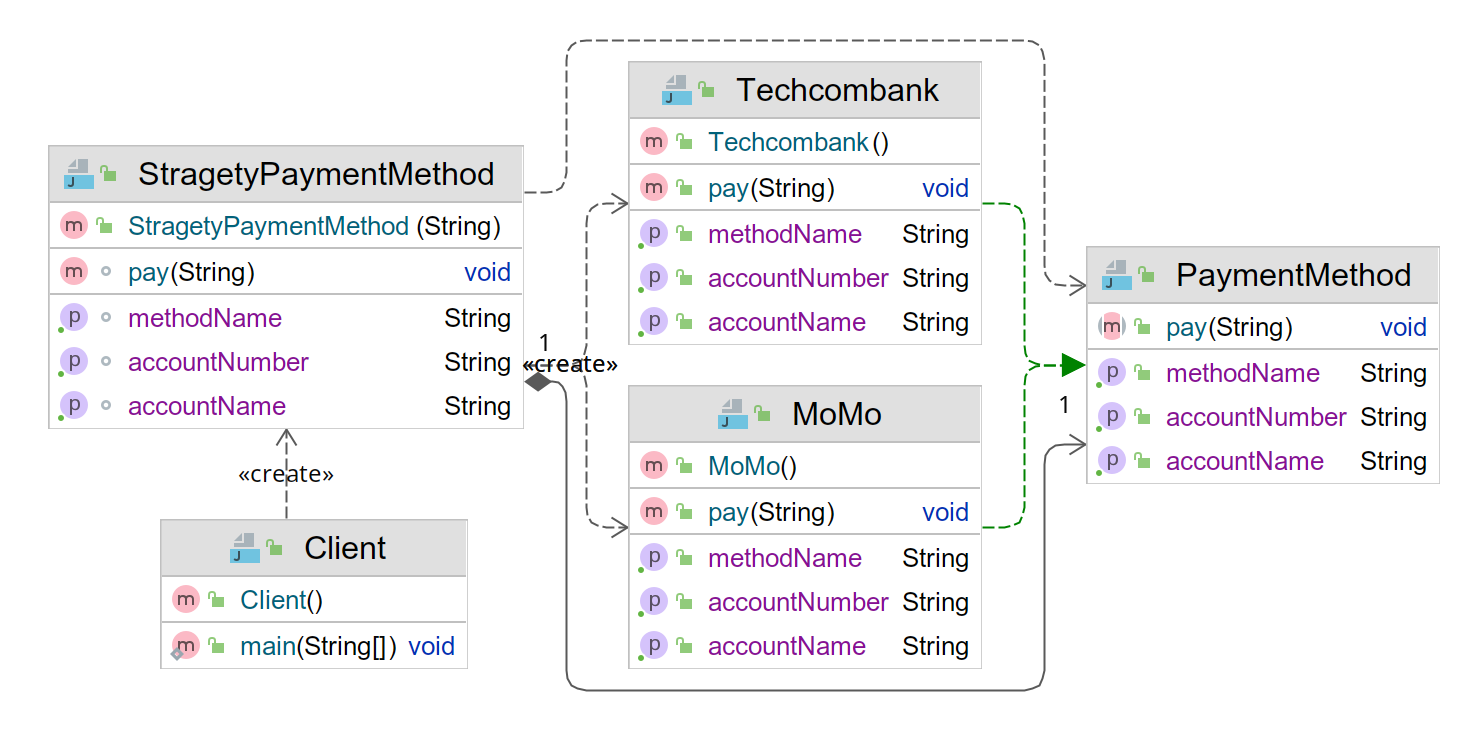
\includegraphics[scale=0.33]{./image/stragety-example.png}
        \end{figure}
    \end{itemize}
    \pagebreak

    \part{PHỤ LỤC}
    \section{Tài liệu tham khảo}
    \begin{itemize}
        \item[1.]\subpara{Slides Bài giảng}
        \item[2.]\subpara{Head First Design Patterns}
        \item[3.]\subpara{https://sourcemaking.com/design-patterns}
        \item[4.]\subpara{https://github.com/LuisBurgs/design-patterns}
        \item[5.]\subpara{https://gpcoder.com/4164-gioi-thieu-design-patterns/}
    \end{itemize}
    \section{Link Project bài báo cáo}
    \begin{itemize}
        \item[1.]\subpara{Link github: \href{https://github.com/blaplafla13th/design-patterns}{https://github.com/blaplafla13th/design-patterns}}
        \item[]\subpara{Project đã bao gồm cả file tex, file pdf, file java, file ảnh kèm theo. Source code sử dụng ở đây là jdk version 17.}
        \item[2.]\subpara{Link Overleaf: \href{https://www.overleaf.com/read/wqxcdvqfhhnx}{https://www.overleaf.com/read/wqxcdvqfhhnx}}
        \item[]\subpara{Bao gồm file latex và ảnh.}
    \end{itemize}
\end{document}
